% NN Builder: user manual. Build: latexmk -pdf nn_builder_manual.tex (pdfLaTeX; no biber needed, the references are a plain bibliography).
\documentclass[11pt,a4paper]{article}

\usepackage[utf8]{inputenc}
\usepackage[T1]{fontenc}
\usepackage{lmodern}
\usepackage[margin=2.3cm]{geometry}
\usepackage{amsmath,amssymb}
\usepackage{booktabs}
\usepackage{tabularx}
\usepackage{longtable}
\usepackage{array}
\usepackage{enumitem}
\usepackage{xcolor}
\usepackage{graphicx}
\graphicspath{{figures/}}
\usepackage{tikz}
\usetikzlibrary{positioning,arrows.meta,fit,calc}
\usepackage{caption}
\usepackage[hidelinks]{hyperref}
\usepackage{url}
\usepackage{fancyvrb}

\definecolor{nnaccent}{HTML}{2F6FDE}
\definecolor{nnconv}{HTML}{D9822B}
\definecolor{nnpool}{HTML}{2A9D8F}
\definecolor{nnnorm}{HTML}{8E5BB5}
\definecolor{nndense}{HTML}{4B5BB5}
\definecolor{nnjoin}{HTML}{C0392B}
\definecolor{nnout}{HTML}{2E8B57}
\definecolor{nntok}{HTML}{0F766E}
\definecolor{nnatt}{HTML}{7C3AED}
\definecolor{nnin}{HTML}{3B6FD8}

\newcommand{\ui}[1]{\textbf{\textsf{#1}}}
\newcommand{\kbd}[1]{\mbox{\fboxsep=1.5pt\fbox{\footnotesize\texttt{#1}}}}
\newcommand{\file}[1]{\texttt{#1}}
\newcommand{\shape}[1]{$(#1)$}
% a screenshot of the application: \screenshot{file}{caption}{label}
\newcommand{\screenshot}[3]{\begin{figure}[htbp]\centering\includegraphics[width=\linewidth]{#1}\caption{#2}\label{#3}\end{figure}}
\newcommand{\note}[1]{\par\smallskip\noindent\fcolorbox{nnaccent!60}{nnaccent!6}{\parbox{\dimexpr\linewidth-2\fboxsep-2\fboxrule}{\small #1}}\par\smallskip}

\tikzset{
  blk/.style={draw, rounded corners=2pt, minimum height=6.5mm, inner sep=3pt, font=\footnotesize\sffamily, line width=0.6pt},
  arr/.style={-{Stealth[length=2mm]}, line width=0.5pt},
}

\setlist{itemsep=2pt, topsep=4pt}
\setlength{\parskip}{4pt}
\setlength{\parindent}{0pt}
\setlength{\emergencystretch}{2em}

\title{\textbf{NN Builder}\\[4pt]\large User manual: using the application, designing a neural network,\\ and the demo architectures explained}
\author{The NN Builder project\\\small\url{https://github.com/varunjha089/NN-Builder}}
\date{5 November 2026 (version 0.3 and the changes after it; see CHANGELOG.md)}

\begin{document}
\maketitle

\begin{abstract}
NN Builder is a desktop application for designing neural networks on a canvas, the way one draws a block diagram. The design is checked
while it is drawn: every connection shows the shape of the tensor it carries, every block shows its output size and parameter count, and
mistakes are explained in plain words on the block itself. A finished design becomes a complete, readable PyTorch training script that also
loads the data (a built-in dataset, Hugging Face or Kaggle), and the application runs it on a GPU somewhere else: a free Kaggle notebook,
a college GPU server over SSH, or an Amazon EC2 instance (including spot instances, which may be interrupted). The computer the application
runs on only designs: it never trains, never downloads datasets and needs no PyTorch.
This manual explains the application screen by screen, walks through designing a network from scratch, gives the arithmetic behind every
number the application shows, explains the fifteen demo architectures (from LeNet-5 to a one-billion-parameter Vision Transformer, plus one
original design), and ends with troubleshooting. References point to the original papers, on arXiv wherever they are published there.
\end{abstract}

\tableofcontents
\newpage

%=====================================================================================================================================
\section{What NN Builder is}

\subsection{The idea}
Building a neural network usually means writing code, running it, and finding out from an error message (or worse, from silently bad
results) that a layer received a tensor of the wrong shape. NN Builder moves that discovery to the moment of design. It is inspired by
visual programming tools such as MIT App Inventor: blocks are placed and connected, and the tool refuses or explains combinations that cannot
work.

Three principles shape the application:
\begin{enumerate}
  \item \textbf{The design computer only designs.} Shapes, parameter counts and the generated code are computed by an engine written in
        Rust inside the application, instantly and offline. No deep-learning library is installed locally, and no dataset is downloaded
        to the design computer.
  \item \textbf{Training happens on a GPU elsewhere, automatically.} One button generates the script, uploads it, prepares the machine
        if needed, starts the run, follows it, and brings the results back.
  \item \textbf{A run does not depend on the connection.} On a server or an EC2 instance the run is started detached; it continues
        when the laptop sleeps, the network drops or the application is closed, and the application reconnects to it later.
\end{enumerate}

\subsection{The workflow at a glance}
\begin{center}
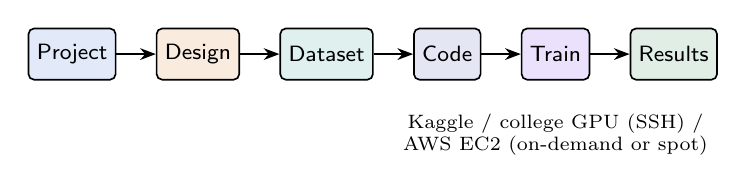
\begin{tikzpicture}[node distance=5mm]
  \node[blk, fill=nnin!15] (p) {Project};
  \node[blk, fill=nnconv!15, right=of p] (d) {Design};
  \node[blk, fill=nnpool!15, right=of d] (ds) {Dataset};
  \node[blk, fill=nndense!15, right=of ds] (c) {Code};
  \node[blk, fill=nnatt!15, right=of c] (t) {Train};
  \node[blk, fill=nnout!15, right=of t] (r) {Results};
  \foreach \a/\b in {p/d,d/ds,ds/c,c/t,t/r} \draw[arr] (\a) -- (\b);
  \node[below=3mm of t, font=\scriptsize, align=center] {Kaggle / college GPU (SSH) /\\ AWS EC2 (on-demand or spot)};
\end{tikzpicture}
\end{center}
The tabs in the top bar follow this order. \ui{Connection}, set apart on the right, holds the tokens and machines that training needs,
and is usually visited once.

\subsection{What it is not}
NN Builder covers image classification and image segmentation. It does not (yet) train on text, audio or tabular data, and it does not
run training on the design computer, even for a tiny network. The generated script, however, is ordinary PyTorch~\cite{paszke2019pytorch}:
it can be copied, read, edited and run anywhere by hand.

%=====================================================================================================================================
\section{Installing, updating and the window}

\subsection{Installing}
Installers are published with every release on GitHub (\url{https://github.com/varunjha089/NN-Builder/releases/latest}):
\begin{itemize}
  \item \textbf{macOS} (Apple silicon): the file ending in \file{\_aarch64.app.zip}. Unzip it and move \file{NN Builder.app} to
        the Applications folder. The application is not signed by Apple, so the first start may need a right-click on the application and
        \ui{Open}.
  \item \textbf{Windows}: \file{NN-Builder\_X\_x64-setup.exe}.
  \item \textbf{Linux}: \file{nn-builder\_X\_amd64.deb} or the portable \file{.AppImage}.
\end{itemize}

\subsection{Automatic updates}
Once a day (if enabled), the application asks GitHub for the latest release. When a newer version exists, a banner appears under the top
bar with \ui{Install and restart}. The download is checked against the SHA-256 checksum published with the release before anything is
replaced. The switch is in \ui{Settings} (and on the Projects page); \ui{Help} $\rightarrow$ \ui{Check for Updates\ldots} checks at once.

\subsection{The top bar}
From left to right: the name, the \ui{Project} button (the current project, or \emph{No project}; it opens the Projects page), a
\ui{not saved} badge and a \ui{Save\ldots} button when the open project is an unsaved demo, the tabs \ui{Design}, \ui{Dataset},
\ui{Code}, \ui{Train}, \ui{Results}, then on the right a summary (``\emph{N params $\cdot$ ready}'' in green, or
``\emph{design has problems}'' / ``\emph{dataset incomplete}'' in red), the day/night button (a moon in day mode, a sun in night mode), the \ui{Settings} button, and \ui{Connection} (a red dot means something is still missing there).

\subsection{Menus and keyboard shortcuts}
\begin{longtable}{@{}p{3.1cm}p{3.3cm}p{8.6cm}@{}}
\toprule
\textbf{Menu} & \textbf{Item (shortcut)} & \textbf{What it does}\\
\midrule\endhead
NN Builder & Settings\ldots\ (\kbd{Cmd+,}) & opens the Settings page\\
File & New Project\ldots\ (\kbd{Cmd+N}) & Projects page, cursor in the name field\\
 & Open Project\ldots\ (\kbd{Cmd+O}) & choose a project folder\\
 & Save Project\ldots\ (\kbd{Cmd+S}) & keeps an unsaved demo as a real project\\
 & Close Project & back to the Projects page with no project open (an unsaved demo is discarded)\\
 & Delete (Projects page) & asks in the row, then moves the project's folder (design, runs, results) to the Trash, from where it can be put back; a missing project is only taken off the list\\
 & New from Demo $\triangleright$ & opens one of the fifteen demo architectures\\
 & Import / Export Design\ldots & reads or writes a design (\file{model.json})\\
 & Export train.py\ldots\ (\kbd{Cmd+E}) & saves the generated training script\\
 & Show Project in Finder (\kbd{Shift+Cmd+R}) & reveals the project folder\\
Edit & Undo (\kbd{Cmd+Z}), Redo (\kbd{Shift+Cmd+Z}) & undo/redo changes to the design (in a text field: the typing)\\
 & Arrange Left to Right (\kbd{Cmd+L}) & lays the canvas out in columns by depth\\
View & Night Mode (\kbd{Shift+Cmd+N}) & switches the neon night theme\\
Connection & Open Connection (\kbd{Shift+Cmd+K}) & the Connection page\\
 & Install Tools\ldots & installs the \file{kaggle} and \file{boto3} helpers\\
Help & Documentation (\kbd{Cmd+?}) & opens this manual (a PDF inside the application)\\
 & Check for Updates\ldots & asks GitHub for a newer release\\
\bottomrule
\end{longtable}

\subsection{Day and night themes, Settings}
The night theme draws panels dark and boxes and text as neon glows; every layer glows in the colour of its kind (Conv2D orange, pooling
teal, normalisation violet, Dense blue, joins red, outputs green, transformer blocks teal and violet). In night mode the Design screen is
split into three separate panels (blocks on the left, canvas in the middle, inspector on the right). Their background colours are chosen in
\ui{Settings} $\rightarrow$ \ui{Night panel colours}: six presets (Midnight, Deep purple, Ocean, Carbon, Forest, Crimson) or a colour
picker per panel, with a live preview; a warning appears for colours so light that neon text becomes hard to read. The theme, the panel
colours and the automatic-update switch are all on the Settings page (Figure~\ref{fig:settings}); Figure~\ref{fig:day} shows the
day theme.

\screenshot{08_settings}{Settings: the theme, the six presets and a colour picker per panel for the night Design screen, a live preview,
and the automatic-update switch.}{fig:settings}
\screenshot{09_design_day}{The Design screen in the day theme (MSG-Former, fitted to the canvas; the layer table on the right).}{fig:day}

%=====================================================================================================================================
\section{Projects}

\subsection{Creating, opening, saving}
A \emph{project} is a folder. The Projects page has two cards side by side:
\begin{itemize}
  \item \ui{New project}: type a name and press \ui{Create} (or Enter). The folder is made in the projects folder shown underneath
        (\ui{change} picks another one).
  \item \ui{Open}: the projects used before, each with its folder, and a field to open any project folder by its path.
\end{itemize}
Every change is saved as it is made; there is no ``save'' step for a normal project.

\screenshot{01_projects}{The Projects page (night theme): New project and Open side by side, then the demo architectures as tiles.}{fig:projects}

\subsection{Demo architectures are unsaved until you save them}
Below the two cards, \ui{Start from a demo architecture} shows the fifteen demos as tiles (the section folds with its arrow). Clicking a
tile opens that network on the canvas as an \emph{unsaved} project: nothing is written to the projects folder. The top bar then shows
\ui{not saved} and \ui{Save\ldots}. Saving (\ui{Save\ldots} or \kbd{Cmd+S}) asks for a name and moves it into the projects folder as a
normal project. An unsaved demo is discarded, without asking, when another demo or project is opened or created, and when the application
quits. This keeps the projects folder free of ``AlexNet demo 2, 3, 4\ldots''. A demo cannot be trained before it is saved, so that runs
always belong to a kept project.

\subsection{What a project folder contains}
\begin{center}
\begin{tabular}{@{}ll@{}}
\toprule
\file{project.json} & name, creation date\\
\file{model.json} & the design: blocks (with their settings and positions) and arrows\\
\file{dataset.json} & the dataset choice\\
\file{train.json} & the training settings\\
\file{runs/<id>/} & one folder per training run (code, metrics, log, results, model)\\
\bottomrule
\end{tabular}
\end{center}
A design can also be exported on its own (\ui{File} $\rightarrow$ \ui{Export Design\ldots}) and imported into another project.

%=====================================================================================================================================
\section{The Design screen}

\subsection{Layout}
\begin{description}
  \item[Blocks (left).] The palette, grouped as \emph{Image} (Conv2D, Depthwise Conv2D, Pool, Global pool, Flatten),
        \emph{Up-sampling} (ConvTranspose2D, Upsample), \emph{Dense and outputs} (Dense, Output, Segmentation output),
        \emph{Normalise / regularise} (BatchNorm, LayerNorm, Dropout, Activation), \emph{Transformer} (To tokens, Class token +
        position, Self-attention, Token pool) and \emph{Branches} (Add, Concat, Multiply). Above them: the
        \ui{Famous architectures} picker and \ui{Arrange left to right}.
  \item[Canvas (middle).] The network, read from left to right. Each block shows its title (with $\times$ for an error and a warning
        sign for a warning), a one-line summary of its settings, and its output shape with its parameter count. Each arrow shows the
        shape of the tensor it carries. Zoom and pan with the trackpad or the controls; a minimap sits in the corner.
  \item[Inspector (right).] With a block selected: its settings, its shape formula with its own numbers, its receptive field, the
        sliding-window animation (convolution and pooling), and the skip-connection tool. With nothing selected: the whole design's
        parameter count, its problems, and the layer table.
\end{description}

\screenshot{02_design_lenet}{The Design screen with LeNet-5: blocks on the left, the network on the canvas (every arrow labelled with its
tensor shape, every block with its output and parameters), and on the right the whole design's summary and the grouped layer table.}{fig:design}

\subsection{Working with blocks}
\begin{itemize}
  \item \textbf{Add:} click a block in the palette; it is added after the selected block (and connected to it).
  \item \textbf{Connect:} drag from a block's right dot to another block's left dot. Add, Concat and Multiply accept several arrows; all
        other blocks take one.
  \item \textbf{Delete:} select a block or an arrow and press Backspace. The Input block cannot be deleted.
  \item \textbf{Move:} drag blocks; \ui{Arrange left to right} (\kbd{Cmd+L}) places them in columns by depth (the longest path from the
        Input), stacking parallel branches in their column.
  \item \textbf{Undo / Redo:} \kbd{Cmd+Z} / \kbd{Shift+Cmd+Z}; changes made within 0.6 seconds of each other count as one step.
  \item \textbf{Copy / paste:} select blocks (Shift-click or drag a box with Shift) and use \kbd{Cmd+C} / \kbd{Cmd+V}: the copies, with the
        arrows between them, appear below the originals, ready to be connected.
  \item \textbf{Residual block after selected:} inserts Conv 3$\times$3 $\rightarrow$ BatchNorm $\rightarrow$ ReLU $\rightarrow$ Conv
        3$\times$3 $\rightarrow$ BatchNorm $\rightarrow$ Add (with a skip from the selected block) $\rightarrow$ ReLU, keeping its size and channels.
  \item \textbf{Collapse repeated blocks ($\times N$):} draws identical consecutive groups as one node, for example the 40 encoder blocks
        of ViT-g/14 as ``Encoder block $\times$40'' (287 blocks become 8). It is a read-only view; double-click the node or press
        \ui{Show every block} to edit again.
\end{itemize}

\subsection{The layer table}
With nothing selected, the inspector lists the layers grouped into stages, each with its output shape, its parameter subtotal and the
receptive field at its end:
\begin{itemize}
  \item \textbf{Input}.
  \item \textbf{Image stages} by resolution (``Stage 2 $\cdot$ 27$\times$27''); a pooling layer, a Dropout after it, and small vector
        layers inside a stage (a squeeze-and-excitation gate) stay with their stage; decoder stages that grow the image are marked with an
        up arrow.
  \item \textbf{Transformers}: \emph{Embedding} (with a patch convolution before it), \emph{Encoder block 1, 2, \ldots}, \emph{Final norm}.
  \item \textbf{Classifier}: the vector layers at the end.
\end{itemize}
Each group shows its contents in block colours (``Conv2D $\times$3, Pool'') and opens with a click (\ui{Expand all} opens all).

\subsection{Famous architectures and the skip-connection tool}
\ui{Famous architectures} replaces the current design with a demo (the previous design is kept as \file{model.previous.json}) and adjusts
the dataset's image size to the one the architecture was made for. The skip-connection tool (inspector, with a block selected) joins an
earlier block's output to the selected block's output with \emph{Add} (a residual connection, as in ResNet~\cite{he2015resnet}) or
\emph{Concat} (as in DenseNet~\cite{huang2016densenet} and U-Net~\cite{ronneberger2015unet}). When the shapes differ, it inserts a
projection: a 1$\times$1 convolution with the right stride (images), a pooling layer, or a Dense layer (vectors).

%=====================================================================================================================================
\section{Designing a network, step by step}

This section builds a small convolutional network for CIFAR-10~\cite{krizhevsky2009cifar} (32$\times$32 colour photos, 10 classes).

\paragraph{1. A project and the data first.}
Create a project ``CIFAR CNN''. Open \ui{Dataset}, choose \ui{Built-in (torchvision)} and \ui{CIFAR-10}. The Input block now says
\shape{3, 32, 32}: three colour channels of 32$\times$32 pixels. (Choosing the data first means every shape shown while designing is the
real one.)

\paragraph{2. A convolution.}
In \ui{Design}, select the Input block and click \ui{Conv2D}. In the inspector set \ui{Filters} to 32 and choose the preset
``3$\times$3, stride 1 (keep size)''. The block shows $\rightarrow$ \shape{32, 32, 32} and 896 parameters
($3\cdot3\cdot3\cdot32$ weights $+$ 32 biases). The arrow from Input shows \shape{3, 32, 32}.

\paragraph{3. Downsampling.}
With the convolution selected, click \ui{Pool}: max pooling 2$\times$2, stride ``same as pool size''. Output \shape{32, 16, 16}, no
parameters. The inspector animates the 2$\times$2 window sliding with stride 2: every window position gives one output value.

\paragraph{4. Repeat, wider.}
Add another Conv2D (64 filters, 3$\times$3, same) and Pool: \shape{64, 8, 8}. A third pair with 128 filters gives \shape{128, 4, 4}.
This is the common pattern: \emph{the image gets smaller and deeper}.

\paragraph{5. From image to vector.}
A classifier needs one vector per image. Two choices:
\begin{itemize}
  \item \ui{Flatten}: \shape{128, 4, 4} $\rightarrow$ \shape{2048}. Keeps the spatial layout, but the next Dense layer then has many weights.
  \item \ui{Global pool} (average): \shape{128, 4, 4} $\rightarrow$ \shape{128}, one number per channel~\cite{lin2013nin}. Far fewer
        parameters, and it works for any image size.
\end{itemize}
Choose Global pool here.

\paragraph{6. The head.}
Add \ui{Dense} (128 units, ReLU), \ui{Dropout} (rate 0.3)~\cite{hinton2012dropout,srivastava2014dropout}, then \ui{Output}. The
Output block reads the number of classes from the dataset (10) and has $128\cdot10+10=1290$ parameters. The top bar now says
``\emph{\ldots params $\cdot$ ready}''.

\paragraph{7. Make it better.}
\begin{itemize}
  \item Insert \ui{BatchNorm}~\cite{ioffe2015batchnorm} after each convolution (set the convolution's activation to \emph{none}, and add
        an \ui{Activation} ReLU after the BatchNorm): faster, more stable training.
  \item Select the second convolution and use the skip-connection tool to add its input to its output (\emph{Add}): a residual block.
        Where the channel counts differ, the tool adds the 1$\times$1 projection for you.
  \item Look at the layer table: it now shows Stage 1 $\cdot$ 32$\times$32, Stage 2 $\cdot$ 16$\times$16, Stage 3 $\cdot$ 8$\times$8,
        Classifier, each with its parameter subtotal.
\end{itemize}

\paragraph{8. Check, then train.}
The \ui{Code} tab shows the generated script; \ui{Train} starts it on Kaggle, a server or EC2 (Section~\ref{sec:train}).

\subsection{When something is wrong}
\label{sec:checks}
A block turns \textbf{red} when the design cannot work (training is blocked) and \textbf{yellow} when it works but probably not as
intended. Blocks after a red block are greyed out (``fix the layer above''); blocks not connected to the Input are faded and ignored.
The reasons are written on the block and in the inspector. The checks include:

\begin{longtable}{@{}p{1.6cm}p{13.4cm}@{}}
\toprule
\textbf{Level} & \textbf{Check (as the application words it, shortened)}\\
\midrule\endhead
error & exactly one Input; exactly one Output (or Segmentation output), and it must be last; no loops\\
error & the image is too small for the window (``use a smaller kernel, padding, or fewer pooling layers before this'')\\
error & Dense / Output on an image: ``add Flatten or Global pool before it''\\
error & an image block (convolution, pooling) after Flatten or after To tokens\\
error & Add with different shapes (``use a 1$\times$1 Conv2D to match channels, or a stride to match sizes'')\\
error & Concat with different heights/widths; Multiply with incompatible shapes\\
error & attention: the token dimension must divide evenly by the number of heads\\
error & BatchNorm on tokens (use LayerNorm); Output on tokens (add Token pool)\\
error & segmentation: the output must return to the mask size (``Upsample / ConvTranspose2D'')\\
error & pooling padding more than half the window; output padding not smaller than the stride (PyTorch rules)\\
error & the dataset has no classes yet\\
warning & the stride does not divide the input evenly: the last rows/columns are ignored\\
warning & stride larger than the window: pixels between windows are skipped\\
warning & ``same'' padding with an even kernel cannot keep the size exactly\\
warning & a very large Dense layer after Flatten (``try Global pool instead'')\\
warning & a block whose result is not used; Flatten on an input that is already flat\\
\bottomrule
\end{longtable}

%=====================================================================================================================================
\section{The arithmetic behind the numbers}
\label{sec:math}

The engine computes everything below exactly as PyTorch does; on every change to the code, an automatic test on GitHub builds hundreds of
random designs (and all demos) in real PyTorch and compares every shape and parameter count with the application's (most recently:
296 designs, 0 differences). A good visual guide to this arithmetic is Dumoulin and Visin~\cite{dumoulin2016guide}.

\subsection{Output size}
For a convolution or pooling layer with input size $n$ (height or width), kernel $k$, stride $s$, padding $p$ and dilation $d$:
\begin{equation}
  n_{\text{out}} = \left\lfloor \frac{n + 2p - d\,(k-1) - 1}{s} \right\rfloor + 1 .
\end{equation}
\begin{itemize}
  \item \textbf{same}: padding chosen so that, with stride 1, $n_{\text{out}}=n$ (for an odd kernel, $p=d(k-1)/2$). With stride $s>1$
        the application computes the explicit padding PyTorch needs (it refuses \texttt{padding="same"} with a stride), giving
        $n_{\text{out}}=\lceil n/s\rceil$.
  \item \textbf{valid}: $p=0$.
  \item \textbf{a number}: that many pixels of zeros on each side.
\end{itemize}
Dilation~\cite{yu2015dilated} spreads the kernel: a 3$\times$3 kernel with dilation 2 covers 5$\times$5 pixels with 9 weights.
For a transposed convolution (up-sampling):
\begin{equation}
  n_{\text{out}} = (n-1)\,s - 2p + d\,(k-1) + p_{\text{out}} + 1 ,
\end{equation}
so a 2$\times$2 kernel with stride 2 exactly doubles the size. Upsample multiplies the size by its scale.

\subsection{Computation}
The Design screen's summary also gives the \textbf{multiply--accumulate operations (MACs) per image}: convolutions (weights $\times$
output positions), dense layers (per token on a sequence) and attention ($4Nd^2 + 2N^2d$); normalisation, activations, pooling and joins
are counted as zero. ResNet-18 at $224\times224$ comes to the usual 1.8\,G.

\subsection{Parameters}
\begin{center}
\begin{tabular}{@{}p{3.9cm}p{6.4cm}p{5cm}@{}}
\toprule
\textbf{Block} & \textbf{Parameters} & \textbf{Example}\\
\midrule
Conv2D & $k_h k_w C_{\text{in}} C_{\text{out}} + C_{\text{out}}$ (bias) & 3$\times$3, 64$\rightarrow$128: 73\,856\\
Depthwise Conv2D & $k_h k_w C_{\text{in}} m + C_{\text{in}} m$ & 3$\times$3, 512 channels: 5\,120\\
ConvTranspose2D & $k_h k_w C_{\text{in}} C_{\text{out}} + C_{\text{out}}$ & 2$\times$2, 512$\rightarrow$256: 524\,544\\
Dense / Output & $n_{\text{in}} n_{\text{out}} + n_{\text{out}}$ & 4096$\rightarrow$4096: 16\,781\,312\\
BatchNorm & $2C$ (scale and shift) & 64 channels: 128\\
LayerNorm & $2D$ & 768 values: 1\,536\\
Self-attention & $4d^2 + 4d$ (query, key, value, output) & $d=768$: 2\,362\,368\\
Class token + position & $d + (N+1)\,d$ & 196 tokens, $d=768$: 152\,064\\
Pool, Global pool, Flatten, Dropout, Activation, joins & 0 & \\
\bottomrule
\end{tabular}
\end{center}
Convolutions followed by BatchNorm are created without a bias in the demos (the BatchNorm shift makes it redundant), as torchvision does.

\subsection{Receptive field}
The receptive field of a block is the size of the input region that one of its output values can see. With $r_0=1$ and $j_0=1$ (the
``jump'', the distance in input pixels between neighbouring outputs), each layer with kernel $k$, dilation $d$ and stride $s$ gives
\begin{equation}
  r_\ell = r_{\ell-1} + d\,(k-1)\, j_{\ell-1}, \qquad j_\ell = j_{\ell-1}\, s .
\end{equation}
The inspector shows it for every block (``one output value here sees 99$\times$99 input pixels''). A network should usually reach a
receptive field about the size of the objects it must recognise; the \emph{effective} receptive field is smaller and concentrated in the
centre~\cite{luo2017erf}.

\subsection{Memory needed for training}
A useful estimate for training with Adam~\cite{kingma2014adam} in mixed precision~\cite{micikevicius2017mixed} is about
\textbf{16 bytes per parameter} before any images: 4 for the weights, 4 for the gradients and 8 for Adam's two running averages. On top
come the activations kept for the backward pass, which grow with the batch size and the image size. Examples: ResNet-18 (11.2 M
parameters) needs about 0.2 GB for its state; ViT-Base (86 M) about 1.4 GB; ViT-g/14 (1.01 B) about 16 GB, more than a 16 GB T4 has. If a
run fails with ``CUDA out of memory'', halve the batch size; beyond that, gradient checkpointing~\cite{chen2016checkpoint} and sharding
the optimizer state over several GPUs~\cite{rajbhandari2019zero} are the standard remedies (not built into NN Builder).

%=====================================================================================================================================
\section{Reference of all blocks}

\begin{longtable}{@{}p{2.9cm}p{3.7cm}p{8.4cm}@{}}
\toprule
\textbf{Block} & \textbf{Shape in $\rightarrow$ out} & \textbf{Settings and notes}\\
\midrule\endhead
Input & $\rightarrow (C,H,W)$ & set by the dataset (channels, height, width)\\
Conv2D & $(C,H,W)\rightarrow(F,H',W')$ & filters, kernel (with a ``square'' link: unlink for height$\times$width), stride, padding (same / valid / number), dilation, activation, bias; presets: 3$\times$3 keep size, 3$\times$3 stride 2 (halve), 1$\times$1 (mix channels), 5$\times$5, 7$\times$7 stride 2 (ResNet stem)\\
Depthwise Conv2D & $(C,H,W)\rightarrow(Cm,H',W')$ & one filter per input channel (channel multiplier $m$); with a following 1$\times$1 Conv2D it forms a depthwise separable convolution~\cite{howard2017mobilenets}\\
ConvTranspose2D & $(C,H,W)\rightarrow(F,H'',W'')$ & learnt up-sampling; filters, kernel, stride, padding, output padding\\
Pool & $(C,H,W)\rightarrow(C,H',W')$ & max or average; pool size; stride (default: same as size); padding\\
Global pool & $(C,H,W)\rightarrow(C)$ & average or max over the whole image\\
Upsample & $(C,H,W)\rightarrow(C,sH,sW)$ & scale, nearest or bilinear; no parameters\\
BatchNorm & same shape & normalises each channel over the batch~\cite{ioffe2015batchnorm}; images and vectors only\\
LayerNorm & same shape & normalises each sample~\cite{ba2016layernorm}; on tokens, over the dimension; on an image, over (channels, height, width)\\
GroupNorm & same shape & normalises each image over groups of channels; independent of the batch, so good for small batches; the channels must divide by the number of groups (often 32)\\
Dropout & same shape & rate: the fraction of values set to zero during training~\cite{srivastava2014dropout}\\
Flatten & $(C,H,W)\rightarrow(CHW)$ & \\
Dense & $(n)\rightarrow(u)$; tokens $(N,D)\rightarrow(N,u)$ & units, activation; on tokens it acts on each token (the transformer MLP)\\
Activation & same shape & ReLU, Leaky ReLU, GELU~\cite{hendrycks2016gelu}, SiLU~\cite{ramachandran2017swish}, sigmoid, tanh\\
Add & equal shapes $\rightarrow$ same & element-wise sum: residual connections~\cite{he2015resnet}\\
Concat & joins along channels & images need equal height and width; the arrow order is the channel order\\
Multiply & see notes & equal shapes; a one-channel map times an image (attention gate~\cite{oktay2018attention}); a per-channel vector times an image (squeeze-and-excitation~\cite{hu2017senet})\\
To tokens & $(C,H,W)\rightarrow(N,D)$ & \emph{patches}: every pixel of the feature map becomes a token of $C$ values ($N=HW$), used after a patch convolution as in ViT~\cite{dosovitskiy2020vit}; \emph{rows}: every image row is a token\\
Class token + position & $(N,D)\rightarrow(N{+}1,D)$ & a learnt class token in front, and learnt position embeddings added\\
Self-attention & $(N,D)\rightarrow(N,D)$ & heads, dropout; multi-head scaled dot-product attention~\cite{vaswani2017attention}\\
Token pool & $(N,D)\rightarrow(D)$ & the class token, the mean of all tokens, or the last one (after an LSTM / GRU)\\
Cross-attention & $(N,D),(M,D_2)\rightarrow(N,D)$ & the first input's tokens attend to the second's (queries; keys and values); heads,
dropout\\
RMSNorm & same shape & per token: divided by its root mean square, times a learnt scale (LLaMA)\\
SwiGLU & same shape & the gated MLP $W_2(\mathrm{silu}(W_1x)\cdot W_3x)$; hidden units\\
Output & $(n)\rightarrow(K)$ & $K$ = number of classes; softmax/cross-entropy is in the training script\\
Segmentation output & $(C,H,W)\rightarrow(K,H,W)$ & a 1$\times$1 convolution giving a class score for every pixel; must match the mask size\\
Early exit & $(n)\rightarrow(K)$ & an extra classifier part way through, trained with the same labels (its loss $\times$ weight); Results
show what stopping confident images there would give\\
Mixture of experts & same shape & a router sends every token to its top $k$ of $E$ expert MLPs; a load-balancing loss keeps all in use\\
Detection output & $(C,h,w)\rightarrow(K{+}4,h,w)$ & anchor-free boxes (CenterNet~\cite{zhou2019centernet}): per cell a score per class, the
box's width and height and the centre's offset; the image must be a whole number of cells (Section~\ref{sec:detection})\\
Conv3D & $(C,T,H,W)\rightarrow(F,T',H',W')$ & a time series: filters, kernel (pixels), dates per window, stride (pixels), padding same
/ valid (Section~\ref{sec:timeseries})\\
Temporal pool & $(C,T,H,W)\rightarrow(C,H,W)$ & the dates of every pixel combined: mean, maximum, or attention (weights learnt per
pixel, as in U-TAE~\cite{garnot2021utae})\\
To sequence & $(C,T,H,W)\rightarrow(T,C)$ & the mean of every date's pixels: one vector per date\\
Conv1D & $(T,D)\rightarrow(T',F)$ & a convolution along a sequence: filters, kernel, stride, padding\\
LSTM, GRU & $(T,D)\rightarrow(T,u)$ & recurrent layers along a sequence~\cite{hochreiter1997lstm}; units, both directions ($2u$ out); Token pool
\emph{last} keeps the last step\\
Subtract & equal shapes $\rightarrow$ same & the first input minus the second, or $|a-b|$: the difference of two branches (Siamese
change detection)\\
Shared weights & as the shared block & runs another block's layer, with the same weights, on its own input of the same shape; the weights
count once (Siamese / twin networks, Section~\ref{sec:siamese})\\
Custom (PyTorch) & declared by the class & runs a class from the design's own PyTorch code (an \texttt{nn.Module} given the input
shape; a \texttt{\# out:} line declares the output shape); the inspector edits the code; checked on the training machine
(Section~\ref{sec:custom})\\
\bottomrule
\end{longtable}

\subsection{Your own layers in PyTorch (Custom block)}
\label{sec:custom}
When a layer is not in the block list (a new attention variant, a gate from a paper, a pixel shuffle), write it in PyTorch. Add a
\ui{Custom (PyTorch)} block (palette: \emph{Your own}) and select it. The inspector shows the design's PyTorch code, shared by all
its Custom blocks, and a \ui{Class} list with the classes in it; \ui{Insert an example} adds a squeeze-and-excitation class to start
from. Each class is an \texttt{nn.Module} at the top level of the code:
\begin{itemize}[nosep]
  \item \texttt{\_\_init\_\_(self, c, h, w)} receives the shape of the block's input (\texttt{t, d} for tokens, \texttt{n} for a vector),
        so the class can size its layers;
  \item a line \texttt{\# out: c * 2, h // 2, w // 2} in the class declares the output shape in those names (without it, the output
        has the input's shape). NN Builder uses it to check and size the rest of the design;
  \item \texttt{forward(self, x)} returns the output. \texttt{torch} and \texttt{nn} are imported; import anything else at the top.
\end{itemize}
The Mac never runs this code. It is copied into \file{train.py} above the network, and on the training machine the one-batch check
compares each Custom block's real output shape with the declared one before any training, stopping with the block's name if they
differ. The parameters of Custom blocks are counted there too (the Design tab's total leaves them out). In the Text tab the code is the
\texttt{python """ \dots{} """} section and the block is \texttt{custom CLASS} (Section~\ref{sec:custom-text}).

The loss can be your own as well: \ui{Loss: your own (Python)} in the Train tab opens a box with \texttt{def custom\_loss(out, y):}
(an example for the task is filled in). \texttt{out} is the network's output for a batch and \texttt{y} the labels as the data gives
them (class numbers; 0/1 per class for multi-label; a class per pixel with $-100$ for unlabelled pixels; the standardised targets for
regression); it returns one number. The validation loss uses it too.

\subsection{Transformer options: masks, positions, LLaMA-style blocks, cross-attention}
\label{sec:transformer-extra}
\ui{Self-attention} has two switches: \ui{causal} (each token sees only itself and the tokens before it, as in a decoder or for a time
series that must not look ahead) and \ui{rotary positions} (RoPE: the queries and keys are rotated by an angle that grows with the
position, so attention depends on how far apart two tokens are; use it with \ui{Positions: none} in Class token + position).
\ui{Positions} can also be fixed sines and cosines (no parameters). \ui{RMSNorm} and \ui{SwiGLU} give LLaMA-style blocks (RMSNorm
$\rightarrow$ attention $\rightarrow$ Add, RMSNorm $\rightarrow$ SwiGLU $\rightarrow$ Add). \ui{Cross-attention} joins two token streams:
the first arrow's tokens ask, the second's are looked at, e.g.\ Sentinel-2 patch tokens attending to Sentinel-1 tokens (mid fusion with
attention instead of Concat), or one date's tokens attending to the others. Concat joins token sequences one after the other. In a
time series, dates with no data at all (every pixel empty) are filled from the dates before and after, so attention needs no mask for
them; a token embedding for text is not part of NN Builder (it trains on images).

\subsection{Frozen layers, LoRA, experts and early exits}
\label{sec:adapters}
\begin{description}[nosep]
  \item[Frozen.] Every block with weights has a \ui{frozen} switch (text: the word \texttt{frozen}): its weights stay as they are, e.g.\
        the first layers of a network started from ImageNet weights. The Design tab shows how many weights are trained and how many frozen.
  \item[LoRA.] Dense and Self-attention have a \ui{LoRA rank}. The layer's own weights are frozen and a low-rank change $B\cdot A$ (rank
        $r$, $B$ starting at zero) is learnt instead~\cite{hu2021lora}: with ImageNet weights and \ui{train only the new layers}, the loaded
        weights stay and only the adapters and the new head learn, a small fraction of the weights. Text: \texttt{dense 64 lora 8},
        \texttt{attention heads 8 lora 4}.
  \item[Mixture of experts.] The \ui{Mixture of experts} block (tokens or vectors) holds $E$ small expert MLPs and a router; every token
        goes to its top $k$ experts, whose outputs are mixed by the router's weights (Switch, Mixtral). Many more weights at the cost of $k$
        experts per token; a load-balancing loss (Switch Transformer, $\times 0.01$) keeps every expert in use. Text: \texttt{moe 8 top 2
        hidden 256}.
  \item[Early exits.] An \ui{Early exit} after a Global pool part way through a classifier is an extra Output trained with the same labels
        (its loss times its \ui{share}). Results list each exit's accuracy and what stopping every image at the first exit that is at
        least 90\,\% sure would give: the accuracy and the share of images leaving at each exit, i.e.\ how much computation could be
        saved. Text: \texttt{exit 0.3}.
\end{description}

\subsection{Several GPUs}
\label{sec:multigpu}
On a machine with several GPUs (a college server, a multi-GPU EC2 instance such as g4dn.12xlarge or g5.12xlarge, a Kaggle notebook with
two T4s) the Train tab's \ui{GPUs} can be \emph{all the machine has} or a number. \file{train.py} then starts one worker per GPU itself
(nothing else changes in how the run is started) and trains with PyTorch's DistributedDataParallel: every worker holds the whole network
and takes its share of every batch, the gradients are averaged after each step, and BatchNorm counts the images of all GPUs. The batch
size stays the total, so the training goes as on one GPU, in about $1/N$ of the time when the data loading keeps up. Worker~0 evaluates,
writes the events, checkpoints and results; the stop button, the spot interruption notice and the timed checkpoints reach every worker
(the run's process forwards them), all stop at the same step, and a resumed run continues at the same batch. With several GPUs a batch
that does not fit is not split automatically (use a smaller batch or \ui{save memory}); a data check uses one GPU. The Kaggle API
cannot choose the T4$\times$2 accelerator: a Kaggle run gets one GPU unless the notebook is set to two. A model too big for one GPU's
memory (FSDP, splitting the weights over the GPUs) is not supported yet.

\subsection{Transformers in NN Builder}
A transformer works on a \emph{sequence of tokens}, shape $(N, D)$: $N$ tokens of $D$ values. To use one on images:
\begin{enumerate}
  \item cut the image into patches with a convolution whose kernel equals its stride (ViT: 16$\times$16, stride 16, $D$ filters), giving
        $(D, H/16, W/16)$;
  \item \ui{To tokens} (patches) turns that map into $N=(H/16)(W/16)$ tokens;
  \item \ui{Class token + position} adds a learnt class token and position information (attention by itself ignores order);
  \item repeat the \emph{encoder block}: LayerNorm $\rightarrow$ Self-attention $\rightarrow$ Add (with the block's input), then
        LayerNorm $\rightarrow$ Dense (GELU, usually $4D$ units) $\rightarrow$ Dense ($D$) $\rightarrow$ Add. Normalising before each
        part (``pre-norm'') trains more stably than after it~\cite{xiong2020prenorm};
  \item a final LayerNorm, \ui{Token pool} (class token), \ui{Output}.
\end{enumerate}

\begin{figure}[htbp]\centering
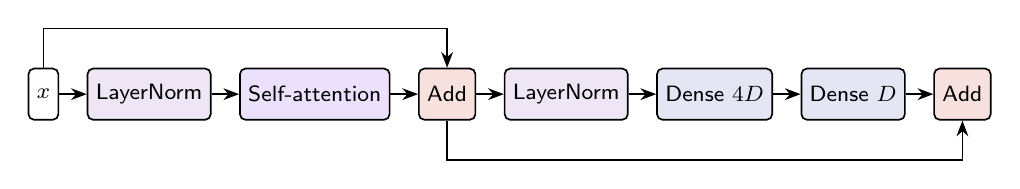
\begin{tikzpicture}[node distance=3.5mm]
  \node[blk] (x) {$x$};
  \node[blk, fill=nnnorm!15, right=of x] (ln1) {LayerNorm};
  \node[blk, fill=nnatt!15, right=of ln1] (at) {Self-attention};
  \node[blk, fill=nnjoin!15, right=of at] (a1) {Add};
  \node[blk, fill=nnnorm!15, right=of a1] (ln2) {LayerNorm};
  \node[blk, fill=nndense!15, right=of ln2] (d1) {Dense $4D$};
  \node[blk, fill=nndense!15, right=of d1] (d2) {Dense $D$};
  \node[blk, fill=nnjoin!15, right=of d2] (a2) {Add};
  \foreach \a/\b in {x/ln1,ln1/at,at/a1,a1/ln2,ln2/d1,d1/d2,d2/a2} \draw[arr] (\a) -- (\b);
  \draw[arr] (x.north) -- ++(0,5mm) -| (a1.north);
  \draw[arr] (a1.south) -- ++(0,-5mm) -| (a2.south);
\end{tikzpicture}
\caption{A pre-norm Transformer encoder block as it is built on the canvas.}
\end{figure}

\subsection{Segmentation}
For segmentation (Dataset $\rightarrow$ \ui{Segmentation}) every pixel gets a class. The network must end with \ui{Segmentation output}
at the size of the masks, so an encoder that shrinks the image needs a decoder that grows it again (ConvTranspose2D or Upsample), as in
U-Net~\cite{ronneberger2015unet}. The training script uses a per-pixel cross-entropy loss and reports pixel accuracy and the mean
intersection over union (mIoU) of the classes.

%=====================================================================================================================================
% The design language (NNB text): included by nn_builder_manual.tex. Every example is a file in examples/ that the tests build
% (crates/core/tests/text.rs, manual_examples_build), so what is shown here works as printed.
\section{Writing designs as text: the NNB language}
\label{sec:text}

Every design can also be written as text, in the \ui{Text} tab. The text and the canvas are two views of the same design and are kept in
step both ways: typing changes the canvas a moment after the text is valid, and a change on the canvas changes the text. This chapter
teaches the language from the first line to functions and loops, then lists every block and every rule.

Why write text at all? A network of fifty blocks is fifty short lines, typed in a minute; every number of every block is visible at once;
repeated parts are written once (\texttt{repeat 40 \{ \dots\ \}}); and the text can be copied into a paper, an e-mail or a chat and pasted
back unchanged (\ui{Copy}, or \ui{File} $\rightarrow$ \ui{Export Design\dots} as a \file{.nnb} file).

\subsection{A first design, line by line}
The smallest useful design is a chain of blocks. LeNet-5 (Section~\ref{sec:demos}) for the $1\times28\times28$ MNIST digits:

\VerbatimInput[fontsize=\small,frame=single,numbers=left,numbersep=6pt,label=\file{lenet5.nnb}]{examples/lenet5.nnb}

\begin{itemize}[nosep]
  \item \texttt{net "LeNet-5"} names the design (optional).
  \item Each further line is one block: a \textbf{label} (\texttt{1}, \texttt{2}, \dots), the \textbf{block} (\texttt{conv},
        \texttt{avgpool}, \dots) and its \textbf{settings} in any order. Left-out settings take the same defaults as the canvas (a
        \texttt{conv} without a kernel is $3\times3$, without an activation it uses ReLU, \dots).
  \item A block takes its input from \textbf{the line above} unless it says otherwise.
  \item \texttt{\#} starts a comment, to the end of the line. Blank lines and indentation do not matter.
  \item The first block is \texttt{input}: its shape comes from the Dataset tab, not from the text. \texttt{output} gets as many
        classes as the dataset has.
\end{itemize}
Typed into the Text tab, this draws the nine blocks on the canvas, each with its label in its header, and the shapes and parameters are
those of Section~\ref{sec:math}: 61\,706 parameters.

\subsection{Settings: words and numbers}
Settings are written the way you would say them. For a convolution, the first plain number is the number of filters, \texttt{5x5} is
the kernel, and words set the rest:

\begin{verbatim}
2 conv 64 3x3                      # 64 filters, 3×3, stride 1, padding "same", ReLU
3 conv 128 3x3 stride 2 pad 1 gelu # stride 2, padding 1, GELU
4 conv 128 1x1 valid none nobias   # no padding, no activation, no bias
5 conv 64 3x3 dil 2                # dilation 2
6 conv filters=64 kernel=7x7 stride=2 padding=3   # any setting as name=value
\end{verbatim}
Every setting also has a \emph{name}\texttt{=}\emph{value} form (the names are those of the inspector), useful when a value is computed
(\texttt{kernel=s+2}, below). A word that a block does not know is an error, never ignored: \texttt{conv 64 stide 2} says
``\texttt{'stide' means nothing for conv (did you mean 'stride'?)}''. A value outside its range (a kernel of 40, 100\,000 filters) is an
error on its block.

\subsection{Connections: \texttt{<-}}
A block with a different input, or with several (Add, Concat, Multiply), names them after \texttt{<-}:

\begin{verbatim}
1 input
2 conv 64 3x3
3 conv 64 3x3 none
4 add <- 2, 3          # residual: the output of block 2 plus that of block 3
5 relu
6 conv 32 1x1 <- 2     # a side branch from block 2 (not from the line above)
7 concat <- 5, 6       # channels joined in this order: 5's first, then 6's
\end{verbatim}
A block may only use blocks above it (a network computes each block once, from the blocks before it), so the text can never contain a
loop. \texttt{<- none} makes a block without input (shown as not connected).

\subsection{Labels}
Labels are names, not positions: \texttt{1, 2, 5, 9} is fine, and so is a word (\texttt{stem conv 32 3x3}, then \texttt{<- stem}). The
label may also be left out: \texttt{conv 32 3x3} on its own gets the next free number. Two lines may not have the same label. The labels
are what the canvas shows in each block's header and what the layer table uses, so canvas, text and table name blocks the same way.

\subsection{Names and arithmetic: \texttt{let}}
\texttt{let} gives a value a name; every number may be an expression of names and numbers with \texttt{+ - * /}, \texttt{//}
(whole-number division), \texttt{\%} (remainder), \texttt{\^{}} (power) and parentheses:
\begin{verbatim}
let w = 32
let depth = 6
2 conv w 3x3
3 conv w * 2 3x3 stride 2
4 dense 2 ^ 10 gelu        # 1024
\end{verbatim}
Changing \texttt{w} changes every block that uses it: the quickest way to try a wider or narrower network.

\subsection{Repeating a group: \texttt{repeat}}
Identical parts are written once. A \texttt{repeat} line has a label, a count and the group in braces; the passes are chained (each
pass takes the previous pass's output), and the line's output is the last pass's last block:
\VerbatimInput[fontsize=\small,frame=single,numbers=left,numbersep=6pt,label=\file{vit\_small.nnb}]{examples/vit_small.nnb}
Inside the braces:
\begin{itemize}[nosep]
  \item blocks have \textbf{local labels} (\texttt{a}, \texttt{b}, \dots); on the canvas they become \texttt{5.1.a} \dots\
        \texttt{5.6.g} (line, pass, block);
  \item \texttt{in} is the group's input (for the first pass, the block above the \texttt{repeat} line);
  \item \texttt{i} is the pass number, 1, 2, \dots: \texttt{conv 32 * i 3x3} gets wider in every pass;
  \item the count may be a name (\texttt{repeat depth}); \texttt{repeat 12 as enc} names the group for readers.
\end{itemize}
This ViT has 49 blocks and 1\,806\,538 parameters at $3\times32\times32$; ViT-g/14 is the same pattern with \texttt{repeat 40} and
16 lines in all.

\subsection{A loop over values: \texttt{for}}
\texttt{for} repeats a group once per value, chained like \texttt{repeat}. A value can be a tuple, for several names at once:
\begin{verbatim}
5 for c in 64, 128, 256 { a conv c 3x3 }
6 for c, s in (64, 1), (128, 2), (256, 2) {
    x conv c 3x3 stride s
    y bn
  }
\end{verbatim}
\texttt{i} is also the pass number in a \texttt{for}.

\subsection{Functions: \texttt{def}}
A function is a group of blocks with values, written once and used many times. It is defined with \texttt{def}, its parameters may have
defaults, and a line calls it like a block:
\VerbatimInput[fontsize=\small,frame=single,numbers=left,numbersep=6pt,label=\file{resnet\_small.nnb}]{examples/resnet_small.nnb}
\begin{itemize}[nosep]
  \item \texttt{basic(c, s)} passes the values by position; \texttt{basic(c)} leaves \texttt{s} at its default; \texttt{basic(c=64, s=2)}
        names them.
  \item Inside the function, \texttt{in} is the input of the call (here the line above the call); the last block is the call's output.
  \item A function may call other functions (up to 16 deep: a function that calls itself is reported).
  \item Functions may be defined anywhere in the text, also below their first use.
\end{itemize}
This network has six residual blocks (66 blocks on the canvas, 791\,338 parameters): about forty lines of text.

\subsection{Several inputs, and reaching into a group}
A call (or a \texttt{repeat} / \texttt{for}) can take several inputs: \texttt{<- 3, 2.3.e} gives the call two, called \texttt{in} and
\texttt{in2} inside. A block made inside a group or a call is named by its path: \texttt{2.3.e} is line 2, pass 3, block \texttt{e} (for a
call: line, then block, as in \texttt{7.u}). Together they make U-Net's skip connections:
\VerbatimInput[fontsize=\small,frame=single,numbers=left,numbersep=6pt,label=\file{unet\_small.nnb}]{examples/unet_small.nnb}
Line 2 builds the encoder as three passes whose width depends on the pass number ($16\cdot2^{i-1}$: 16, 32, 64); lines 4--6 each take
the block above and the matching encoder output (25 blocks, 482\,050 parameters for $64\times64$ images and two classes).

\subsection{Every block}
\begin{longtable}{@{}p{3.6cm}p{5.6cm}p{5.8cm}@{}}
\toprule
\textbf{Block (other words)} & \textbf{Example} & \textbf{Settings (default)}\\
\midrule\endhead
\texttt{input} & \texttt{1 input} & none: the shape is the dataset's\\
\texttt{conv} (\texttt{conv2d}) & \texttt{conv 64 3x3 stride 2 pad 1 gelu} & filters (32), kernel \texttt{KxK} or \texttt{K} (3), \texttt{stride} (1), \texttt{pad} n / \texttt{same} / \texttt{valid} (same), \texttt{dil} (1), activation (relu), \texttt{nobias}\\
\texttt{dwconv} (\texttt{dwconv2d}) & \texttt{dwconv x2 3x3 stride 2} & multiplier \texttt{x}n (1), kernel, stride, padding, activation, \texttt{nobias}\\
\texttt{convT} (\texttt{convtranspose}) & \texttt{convT 64 2x2 stride 2 none} & filters (32), kernel (2), stride (2), \texttt{pad} (0), \texttt{outpad} (0), activation (relu)\\
\texttt{maxpool}, \texttt{avgpool} (\texttt{pool}) & \texttt{maxpool 3x3 stride 2 pad 1} & size (2), \texttt{stride} n or \texttt{size} (= size), \texttt{pad} (0)\\
\texttt{global\_pool} (\texttt{gap}) & \texttt{global\_pool max} & \texttt{avg} / \texttt{max} (avg)\\
\texttt{upsample} & \texttt{upsample x2 bilinear} & scale \texttt{x}n (2), \texttt{nearest} / \texttt{bilinear}\\
\texttt{bn}, \texttt{ln}, \texttt{gn} & \texttt{gn 8} & GroupNorm: groups (8; must divide the channels)\\
\texttt{dropout} & \texttt{dropout 0.3} & rate (0.25)\\
\texttt{flatten} & \texttt{flatten} & none\\
\texttt{dense} (\texttt{linear}) & \texttt{dense 128 gelu} & units (128), activation (relu)\\
\texttt{relu}, \texttt{gelu}, \texttt{silu}, \texttt{tanh}, \texttt{sigmoid}, \texttt{leaky\_relu} & \texttt{gelu} & an activation block\\
\texttt{add}, \texttt{concat} (\texttt{cat}), \texttt{mul} (\texttt{multiply}) & \texttt{add <- 2, 5} & two or more inputs; Concat joins channels in the order given\\
\texttt{to\_tokens} & \texttt{to\_tokens patches} & \texttt{patches} (every pixel a token) / \texttt{rows}\\
\texttt{cls\_pos} & \texttt{cls\_pos} & class token + position embedding; \texttt{nocls}: positions only\\
\texttt{attention} (\texttt{attn}) & \texttt{attention heads 8 drop 0.1} & \texttt{heads} (4; must divide the token width), \texttt{drop} (0)\\
\texttt{token\_pool} & \texttt{token\_pool mean} & \texttt{cls} / \texttt{mean} (cls)\\
\texttt{output}, \texttt{seg\_output} & \texttt{output} & none: classes from the dataset\\
\bottomrule
\end{longtable}
The activation words after a \texttt{conv}, \texttt{dwconv}, \texttt{convT} or \texttt{dense} set its activation (\texttt{none}: without);
on their own line they are an Activation block. Block words may be written in capitals (\texttt{Conv}); the text the application prints
uses the short lower-case words.

\subsection{The rules in brief}
\begin{verbatim}
net "name"                                   name of the design (optional)
let NAME = EXPR                              a named value
def NAME(P, Q = EXPR) { LINES }              a function (P, Q: parameters; Q has a default)
LABEL BLOCK SETTINGS [<- REF, REF]           one block; without <- it takes the line above
LABEL NAME(EXPR, Q=EXPR) [<- REF, REF]       a function call (inside: in, in2, ...)
LABEL repeat EXPR [as NAME] [<- REF] { LINES }       passes chained; i = pass number
LABEL for A, B in (EXPR, EXPR), ... [<- REF] { LINES }
REF:  a label | in | in2 | a path like 5.2.b    EXPR: numbers, names, + - * / // % ^ ( )
\end{verbatim}

\subsection{Mistakes and what the application says}
A text with a problem is not applied: the canvas keeps the last valid design, the status says ``not applied'', the line number in the
gutter turns red and the message below the text names the line (click it to jump there). Typical messages:
\begin{longtable}{@{}p{4.6cm}p{10.4cm}@{}}
\toprule
\textbf{Written} & \textbf{Message}\\
\midrule\endhead
\texttt{conv 64 3x3 stide 2} & 'stide' means nothing for conv (did you mean 'stride'?)\\
\texttt{convv 64 3x3} & unknown block 'convv' (did you mean 'conv'?)\\
\texttt{add <- 2, 7} (no line 7 above) & '7': there is no block '7' above this line (a block may only use blocks above it)\\
two lines labelled \texttt{2} & the label '2' is used twice\\
\texttt{dense 10 pad 1} & 'pad' means nothing for dense\\
\texttt{conv 8 3x3 filtrs=4} & conv has no setting 'filtrs' (its settings: activation, bias, dilation, filters, kernel, padding, stride)\\
\texttt{conv 8 3x3 99} & what is the number 99? write it as name=value (e.g.\ filters=99)\\
a \texttt{\{} without \texttt{\}} & a '\{' is not closed with '\}'\\
\texttt{f(1, 2)} for \texttt{def f(c)} & 'f' takes 1 value(s), more were given\\
\texttt{repeat k} without \texttt{let k} & repeat: 'k' is not a number\\
\texttt{repeat 5000 \{ \dots\ \}} too large & 5000 passes × 7 blocks = 35000 blocks, more than the 13000 a design may have (Settings → Design size \dots). At most 1856 passes fit here.\\
\bottomrule
\end{longtable}
Shape problems (an Add of different shapes, a kernel larger than the image) are found by the same checks as on the canvas and listed under
the text with the line of their block; click \emph{block 5.2.a} to see it selected on the canvas. \kbd{Cmd}-click on any label in the text
also selects its block.

\subsection{How the text and the canvas stay in step}
\begin{itemize}[nosep]
  \item \textbf{Typing:} a quarter of a second after the last key, a valid text replaces the design (one undo step). Blocks keep their
        place on the canvas when their label and kind stay the same; new blocks are placed next to their input.
  \item \textbf{Moving blocks} on the canvas keeps the text exactly as written.
  \item \textbf{Changing a setting} of a block that has its own line rewrites only that line (its label, inputs and comment stay).
  \item \textbf{Adding, removing or connecting} blocks of plain lines changes only those lines: a new block gets the next free number and
        goes after its input; a line that took ``the line above'' gets an explicit \texttt{<-} when that changed; a block inserted in front
        of a function call or loop becomes its input. Names, functions, loops and comments stay.
  \item \textbf{Changing a block that a function or loop made} would change every call, so the text is printed again from the blocks:
        identical consecutive groups become \texttt{repeat}, the rest plain lines. \kbd{Cmd+Z} brings the hand-written text back.
  \item \ui{Format} prints the text again from the blocks on purpose; \ui{Copy} copies it.
\end{itemize}
In the layer table, the blocks of one \texttt{repeat}, \texttt{for} or call line form one group named after the line.

\subsection{A design that uses everything}
\file{doc/examples/everything.nnb} in the repository is a hybrid CNN and Transformer written only as text: functions calling functions
with defaults and named values, a function with two inputs, \texttt{for} with tuples, \texttt{repeat} with \texttt{i}, \texttt{let} and
every operator, paths into loop passes, a left-out label, comments, and every block kind except the segmentation output (89 blocks,
186\,086 parameters, no warning at $3\times32\times32$). The test suite builds it and every example of this chapter, and GitHub Actions
compares its layers with real PyTorch.


%=====================================================================================================================================
\section{The Dataset tab}

Only the \emph{description} of a dataset is read on the design computer; the images are downloaded on the GPU machine when training starts
(and cached there in \file{\textasciitilde/.nn\_builder/data}).

\screenshot{05_dataset}{The Dataset tab with built-in CIFAR-10, as MSG-Former opens (the demo picks the built-in set that fits its
input, so nothing is resized).}{fig:dataset}

\paragraph{What data NN Builder reads.} Every kind, with a picture of such data and the Dataset tab set up for it, is in
Section~\ref{sec:data-kinds}.

\begin{center}\small
\begin{tabular}{@{}p{0.27\linewidth}p{0.2\linewidth}p{0.45\linewidth}@{}}
\toprule
Data & Sources & Task and files \\
\midrule
MNIST, Fashion-MNIST, CIFAR-10 & built-in & classification \\
Pictures (PNG, JPEG, \dots; grey or colour) & Hugging Face, Kaggle, own files & classification: a label column, or one folder per class \\
Pictures + masks & Hugging Face, Kaggle, own files & segmentation: a mask column, or images and masks with the same names \\
Satellite / multispectral images (Sentinel-2, any bands) & Kaggle, own files & GeoTIFF or \file{.npy}, 1--32 bands; classification,
  multi-label, segmentation \\
Radar (Sentinel-1 VV, VH) & Kaggle, own files & as above; linear or dB \\
Large exported scenes + label image (Google Earth Engine) & own files, Kaggle & segmentation: cut into tiles \\
Several classes per image (BigEarthNet) & own files, Kaggle, Hugging Face & multi-label: a CSV (or a list column) \\
Two sensors for the same places (S1 + S2) & own files, Kaggle & fusion: two band groups, early or mid \\
\bottomrule
\end{tabular}
\end{center}

\subsection{Built-in datasets}
MNIST (handwritten digits, $1\times28\times28$)~\cite{lecun1998gradient}, Fashion-MNIST (clothing, $1\times28\times28$)~\cite{xiao2017fashion}
and CIFAR-10 (photos, $3\times32\times32$)~\cite{krizhevsky2009cifar}, ten classes each, downloaded by torchvision on the GPU machine.
\ui{Resize the images} enlarges them for networks made for larger inputs (for example 224$\times$224 for AlexNet); the number of channels
can be changed as well (grey images repeated into three channels).

\subsection{Hugging Face}
Type a dataset id (\texttt{owner/name}) and press \ui{Read info}: the application reads its configurations, splits, columns and first
rows from the public datasets-server API, without downloading~\cite{lhoest2021datasets}. Then choose:
\begin{itemize}
  \item \ui{Config} and \ui{Training split} (with its number of rows);
  \item \ui{Test split}: a separate split, or ``10\% of the training split'' (a fixed, seeded split);
  \item \ui{Image column} and \ui{Label column}: the column that holds the pictures (an \emph{Image} feature) and the one that holds the
        class (a \emph{ClassLabel} feature, whose class names fill the class list).
\end{itemize}
Gated or private datasets need a Hugging Face token (Connection tab), which the run can copy to the machine.

\note{\textbf{Only image datasets work.} A text corpus such as \texttt{HuggingFaceFW/fineweb-edu} (web pages and their metadata) has no
image column and no class column: the image and label columns then point at unrelated text, the class list stays empty, and the design
is marked as having problems. Use datasets such as \texttt{uoft-cs/cifar10}, \texttt{ylecun/mnist} or \texttt{food101}. The Dataset tab
now says so at once when a dataset has no image column.}

After \ui{Read info}, the tab also shows the \textbf{class balance} of the training split (counted by Hugging Face's dataset viewer) with a
warning when the largest class has more than three times the images of the smallest, and \ui{Show 8 example images} fetches just eight
pictures to check that the right columns are chosen (the dataset itself is still downloaded only on the GPU machine).

\subsection{Kaggle}
Type the dataset slug (\texttt{owner/name}); with the Kaggle token stored, the application lists its files and recognises the common
layout of \emph{one folder per class}. Set the training folder (and optionally a test folder; otherwise 10\% of the training images are
kept for testing) and the class names (the folder names, in order). On Kaggle the dataset is attached to the notebook; on a server or EC2
it is downloaded with the Kaggle tool, which needs the token on that machine (the Train tab offers to copy it there).

\subsection{Segmentation data}
Hugging Face: an image column and a \ui{Mask column}. Kaggle: an \ui{Images folder} and a \ui{Masks folder} whose files have the same
names. The class list maps mask values to classes (value 0 is the first class; with two classes any non-zero pixel is the second).

\subsection{Image size and classes}
\ui{Image height}, \ui{Image width} and \ui{Channels} set the shape of the Input block; images are resized to it. The class names, one per
line in label order, set the Output block's size.

\subsection{Satellite images: Sentinel-2, Sentinel-1 and other bands}
\label{sec:bands}
Multispectral and radar images have more than three bands and values that are not 0--255 colours, so they are read as arrays, not as
pictures. A Kaggle dataset with one folder per class of GeoTIFF (\file{.tif}, \file{.tiff}) or \file{.npy} files works, as in
EuroSAT-MS. Choose it as usual (\ui{Read files}, the training folder), then under \ui{Image bands}:
\begin{itemize}[nosep]
  \item \ui{Sentinel-2 (13 bands)}: the files' band order is filled in as EuroSAT-MS stores it (B01 \dots\ B12, then B8A; correct it if
        the dataset's description says otherwise). Tick the bands the network should see, or use a preset: all 13, the ten 10\,m and 20\,m
        bands, true colour (B04 B03 B02), or colour and near infrared. Each band shows its wavelength and resolution.
  \item \ui{Sentinel-1 radar (VV, VH)}: the two polarisations; tick \ui{convert to decibels} when the files hold linear backscatter
        (values around 0.01--0.5), since a network learns radar much better in dB.
  \item \ui{other bands}: type the bands of the files in their order and tick the ones to use.
\end{itemize}
The Input block then has as many channels as bands are ticked (up to 32), and the first convolution's parameters follow (13 bands into a
$3\times3$ convolution with 16 filters: $13\cdot9\cdot16+16 = 1\,888$). On the GPU machine \file{train.py}:
\begin{itemize}[nosep]
  \item reads each file (bands first or last), picks the ticked bands by name, converts Sentinel-1 to dB if asked, and resizes to the image
        size of the Dataset tab;
  \item measures the mean and spread of every band on up to 256 training images and normalises each band with its own values (kept in
        \file{band\_stats.json}, so a resumed run normalises the same way);
  \item augments with horizontal / vertical flips and quarter turns (a satellite image has no ``up''), when flips or rotation are ticked
        in the Train tab;
  \item shows the result pictures as composites: true colour (B04 B03 B02) for Sentinel-2, VV / VH / VV$-$VH for Sentinel-1, else the
        first three bands, each stretched between its 2nd and 98th percentile.
\end{itemize}
\textbf{ImageNet weights with bands.} \ui{Start from ImageNet weights} (Train tab) also works for satellite images: the first
convolution's red, green and blue filters go to B04, B03 and B02 (matched by name), every other band gets the mean of the three, and all
are scaled by $3/C$ for $C$ bands so the layer's output keeps its size; the rest of the network loads as usual. The images are still
normalised per band (not with ImageNet's colour statistics).

\textbf{Hugging Face.} A Hugging Face dataset whose image column holds band arrays (an array feature, or GeoTIFF / \file{.npy} bytes)
is read the same way: choose the bands under \ui{Image bands} (type the band order, since it cannot be read on the Mac). Classification,
multi-label (a list column) and segmentation (a mask column) work; two band groups need files (own files or Kaggle).

Several classes per image (Section~\ref{sec:multilabel}) and Sentinel-1 with Sentinel-2 (Section~\ref{sec:fusion}) are below.
GitHub Actions trains on generated Sentinel-2 (mixed \file{.tif} and \file{.npy}) and Sentinel-1 folders on every change and checks the
bands, the statistics and the accuracy; it also trains on every layout of the next section.

\subsection{Your own files, e.g.\ Sentinel-1/2 from Google Earth Engine}
\label{sec:own-files}
Sentinel data is usually exported from Google Earth Engine (GEE) to Google Drive and downloaded, so it is not on Kaggle or Hugging Face.
Choose \ui{Source: My own files}, then the folder (\ui{Choose\dots}) and \ui{Read folder}. The app lists the files, finds class folders,
and reads the first GeoTIFF's header: its size, number of bands and, when GEE or GDAL wrote them, the band names, which fill
\ui{Bands in the files} by themselves (nothing is opened beyond the header, and nothing in the folder is changed).
\begin{description}[nosep]
  \item[Where the files are.] \ui{on this Mac}: when a run starts, the folder is copied to the training machine
        (\file{\textasciitilde/.nn\_builder/data/local/nnb-<folder>-<code>}, with rsync, so only the first time and after a change), or, for
        Kaggle, uploaded under your account as a \emph{private} Kaggle dataset of the same name and attached to the notebook (again only
        when it changed; the folders go up as zip files, which Kaggle unpacks). \ui{already on the training machine}: give its path there
        (e.g.\ a large export copied to the college server yourself); nothing is copied, and Kaggle cannot be used.
  \item[In the cloud.] The training machine (or the Kaggle notebook) fetches the files itself, so a large Earth Engine export never passes
        through the Mac: \texttt{gs://bucket/folder} (Earth Engine's Cloud Storage export: in the export script choose \ui{Export to: Cloud
        Storage}; a private bucket needs a service-account key, Connection tab, which is copied to an SSH or AWS machine with the other
        tokens; Kaggle notebooks read public buckets only), a Google Drive folder or file shared as ``anyone with the link'' (fetched with
        \texttt{gdown}: at most 50 files per folder, a zip is unpacked), or \texttt{rclone:remote:path} for rclone set up on the machine
        (any of its 70 storage services, Drive included). The files are kept in the machine's data folder; a later run fetches only what
        is new.
  \item[Classification.] One subfolder per class (\file{forest/}, \file{water/} \dots) of \file{.tif} or \file{.npy} patches, or ordinary
        pictures. An optional test folder; else 10\,\% of the images.
  \item[Segmentation: images + masks.] An images folder and a masks folder with the same file names (a mask may add \file{\_mask}); masks
        may be PNG, GeoTIFF or \file{.npy} with class numbers 0, 1, 2 \dots
  \item[Segmentation: a large image and a label image.] What GEE exports for a region: one image (possibly split into several files named
        \file{scene-0000000000-0000000000.tif} \dots) and a label image on the same grid with the same file names (in another folder). The
        images are cut into tiles of the image size; a tile is used when at least half of its pixels have data and at least one has a
        class. \ui{Test tiles}: 10\,\% at random (quick, but neighbouring tiles are alike, so the score is optimistic), the eastern
        tenth of every image with one column of tiles left out between it and the training tiles (\emph{strip}: no test tile touches a
        training tile), or a test region exported separately (\emph{files}: the most honest). The arrays are kept as \file{.npy} files in the data folder and read with memory mapping, so a
        scene larger than the memory works.
\end{description}
GEE's conventions are handled: band names B1 \dots\ B9 are the same as B01 \dots\ B09 everywhere in the app (\ui{Earth Engine SR (12,
B1 \dots\ B12)} sets that band order; the surface-reflectance collection has no B10); empty (masked) pixels written as NaN are left out
of the band statistics and filled with the band's mean; label values that are not a class (no data, 255, negative) are left out of the
loss and of the scores; and Sentinel-1 from \texttt{COPERNICUS/S1\_GRD} is already in dB: such files are recognised by their negative
values and not converted again, even with \ui{convert to decibels} ticked.

\subsection{Several classes per image (multi-label)}
\label{sec:multilabel}
In benchmarks such as BigEarthNet a patch can be forest \emph{and} water \emph{and} farmland at once. Choose \ui{Task: Multi-label}.
The labels come from a CSV file (own files or Kaggle): one row per image, a file column (\texttt{file}, \texttt{image}, \texttt{name},
\texttt{path}, \texttt{patch\_id} \dots; with or without the extension, relative to the CSV's folder or the images folder) and either a
labels column with the classes separated by \texttt{;} \texttt{,} \texttt{|} or spaces, or one 0/1 column per class. \ui{Read labels}
reads the class names and how many images have each. From Hugging Face, choose a column that is a list of class labels. Rows that name
a missing file are left out (with a warning). A \texttt{split} column (\texttt{train} / \texttt{validation} / \texttt{test}) is used as
given instead of a random split.

\textbf{BigEarthNet v2 as it is downloaded.} Each patch is a folder of single-band GeoTIFFs (\file{<patch>/<patch>\_B02.tif} \dots, the
20\,m and 60\,m bands at their own sizes) below a tile folder, and the labels are in \file{metadata.parquet} (a list of class names per
patch, the split, and \texttt{s1\_name}, the matching Sentinel-1 patch). Choose \ui{BigEarthNet (19 classes, metadata.parquet)}, set the
\ui{Images folder} to the Sentinel-2 folder, and for fusion add Sentinel-1 as the second band group with its folder: the patch folders are
found below them, every band is brought to the largest band's size, and \texttt{s1\_name} pairs the two sensors. Parquet tables are read
on the training machine only (the class names come from the preset or are typed).

The network ends in the ordinary Output block, one score per class, but every class is its own yes/no: the score goes through a sigmoid,
a class is predicted when it is at least 50\,\%, and the loss is binary cross-entropy summed over the classes (label smoothing pulls the
targets towards 0.5). The run reports micro F1 (every image--class decision together; shown where accuracy usually is), macro F1 (the
classes averaged, so rare classes count as much as common ones), mean average precision (mAP: how well each class's scores rank its
images, independent of the threshold) and exact match (every class of an image right). Results lists precision, recall, F1 and AP per
class, and the sample pictures mark each class as right, wrong or missed.

\subsection{Numbers per image (regression)}
\label{sec:regression}
To predict a quantity instead of a class (above-ground biomass, canopy height, crop yield, soil moisture of a plot), choose \ui{Task:
Regression}. The numbers come from a CSV file next to the images (own files or Kaggle): one row per image, the same file column as for
multi-label, and one numeric column per target. \ui{Read labels} lists the columns that hold a number in every row, with their range;
tick the targets (one or several). From Hugging Face, tick the numeric columns of the table. Rows whose target is empty or not a number
are left out with a warning; a \texttt{split} column is used as given.

The Output block gives one number per target (no softmax). Before training the run measures every target's mean and spread on the
training images, and the network learns the targets standardised (mean 0, spread 1), so targets of very different sizes train equally
well. \ui{Loss} in the Train tab: \emph{mean squared error} (MSE, the default; large errors count most), \emph{L1} (mean absolute error;
less swayed by a few wild values) or \emph{Huber} (squared for errors below one standard deviation of the target, linear above). The
scores are in the targets' own units: R$^2$ (the share of the targets' variation the network explains: 1 is perfect, 0 is no better than
always predicting the mean; shown where accuracy usually is, and what early stopping on ``validation R$^2$'' watches), MAE (mean absolute
error) and RMSE (root mean squared error), per target and averaged. Results shows a predicted-against-true scatter plot per target and
sample images with both numbers. \file{model.pt} outputs the standardised numbers; \file{target\_stats.json} next to it holds each
target's mean and standard deviation (value $=$ output $\times$ std $+$ mean). Flips and rotations are fine for quantities that do not
depend on direction. A number for every pixel (a canopy height map) is not supported yet.

\subsection{Several outputs (multi-task)}
\label{sec:multitask}
One network can predict several things about the same image at once: the land-cover class \emph{and} the biomass, or the crop type
\emph{and} whether the field is irrigated. The shared layers then learn features useful for all of them, which often helps the smaller
tasks. In the Dataset tab, \ui{Extra outputs (multi-task)} $\rightarrow$ \ui{Add an extra output}, for each one:
\begin{itemize}[nosep]
  \item a \ui{name} (shown in the results), what it \ui{Predicts} (one class, several classes, or numbers), and its column(s) of the
        labels table: the class column; the labels column (several classes; empty when they are 0/1 columns); or the number columns;
  \item for classes, the class names in label order; its \ui{Loss} (cross-entropy or focal; binary cross-entropy; MSE, L1 or Huber); and
        its \ui{Weight}: the total loss is the main task's plus each extra output's times its weight.
\end{itemize}
The values come from the labels table next to the images (own files or Kaggle: the same CSV / TSV / Parquet as for multi-label and
regression; with the main task \emph{classification} the image's class is its folder, or the \ui{Main task's class column}), or from
columns of a Hugging Face dataset. Rows without a usable value for an output are left out, with a warning.

In the Design tab each output gets its own Output block: select an Output and choose \ui{Output for} (the main task, 1, 2, \dots; in
text \texttt{output 1}). Usually they share the body of the network and each has a small branch of its own (a Dense or two) before its
Output. The network returns all outputs; the run reports the main task as usual (and its score decides early stopping and the best
epoch) and every extra output in a table: accuracy, micro F1 and mAP, or R$^2$, MAE and RMSE per number, in the numbers' own units. The
Train tab's chart draws each output's validation score.

\subsection{Object detection (boxes)}
\label{sec:detection}
To find and count objects (ships, cars, buildings, trees, animals) with a box around each, choose \ui{Task: Object detection}. The data
are an \ui{Images folder} and a \ui{Labels folder} with one text file per image of the same name (\file{im17.png} and \file{im17.txt}):
one line per box, \texttt{class cx cy w h}, the class number (0 = the first line of the class list) and the box's centre, width and
height as fractions of the image. This is the YOLO format that Roboflow, CVAT and most converted datasets offer; an image without a label
file has no object. Pictures and multiband files both work; 10\,\% of the images are the test data; horizontal and vertical flips move
the boxes with the image.

The network ends in a \ui{Detection output} on a feature map, typically a quarter or an eighth of the image size (two or three
$2\times2$ pools or stride-2 convolutions; the image must be a whole number of cells). For every cell it gives a score per class (is an
object's centre here?), the box's width and height in cells and the centre's offset inside the cell: the anchor-free CenterNet
design~\cite{zhou2019centernet}. Training draws every box as a Gaussian peak on its class's map and uses CenterNet's loss (a focal
loss on the peaks, L1 on size and offset). The boxes found are the peaks of the scores; the run reports mAP@0.5 (a box counts when it
overlaps a true one by at least half, IoU $\ge 0.5$) and mAP@0.5:0.95 (stricter overlaps, as COCO), with the AP of every class, and Results
draws the boxes found (score $\ge$ 30\,\%) and the true ones on test images. Not yet: rotated boxes (DOTA's oriented format), COCO JSON
labels, very large scenes cut into tiles with their boxes, and non-maximum suppression across classes.

\subsection{Time series of satellite images}
\label{sec:timeseries}
A field's crop shows in \emph{when} it greens up and is harvested, more than in any single image. A time series gives the network the
same place at several dates. In the Dataset tab, after choosing the bands, tick \ui{a time series} and give the \ui{dates per sample}.
Each file then holds one place at all its dates: a \file{.npy} of shape (dates, bands, height, width) (or (dates, height, width, bands)),
or a GeoTIFF whose bands go date by date: all bands of the first date, then of the second, \dots{} (as Earth Engine exports a stack of
monthly composites, \texttt{ee.ImageCollection.toBands()}). Class folders, a labels table (multi-label, regression, extra outputs) and
images + masks (a crop-type map) all work; every band is normalised over all its dates, every date is resized like an image, and flips
and turns apply to all dates alike. The result pictures show the median of the dates.

The Input is then $(C, T, H, W)$: bands, dates, height, width. Image blocks do not take it directly; the Time series blocks do:
\begin{itemize}[nosep]
  \item \ui{Conv3D} convolves over neighbouring dates and pixels at once (\emph{dates per window}, e.g.\ 3);
  \item \ui{Temporal pool} combines the dates of every pixel into one image $(C, H, W)$: the mean, the maximum, or \emph{attention}: a
        score for every date and pixel from the pixel's channels, a softmax over the dates, and the weighted sum (the idea of
        U-TAE~\cite{garnot2021utae}). After it every 2-D block works: convolutions, a U-Net decoder, a Segmentation output for a crop map;
  \item \ui{To sequence} takes the mean of every date's pixels, one vector per date $(T, C)$: the time series of the whole patch. Then
        \ui{Conv1D}, \ui{LSTM} and \ui{GRU} work along the dates, and so do the transformer blocks (Class token + position,
        Self-attention, Token pool), which gives a small temporal transformer (as in TSViT~\cite{tarasiou2023tsvit}). Token pool's
        \emph{last} keeps the last step of a recurrent layer.
\end{itemize}
Both kinds of path can start from the same Input and be joined (\file{doc/examples/timeseries.nnb}). BatchNorm, Dropout, the activations,
Add / Subtract / Multiply, Concat (equal dates and size), Flatten and Global pool work on a time series too. Not yet: a date per image
(the dates are taken as evenly spaced), missing dates, a second band group with a time series, Hugging Face time series, the Earth
Engine script for a time stack.

\subsection{Shared weights: Siamese networks and change detection}
\label{sec:siamese}
A Siamese (twin) network looks at two images with the \emph{same} layers, so that both are described in the same terms, and then
compares the two descriptions: has this field been built on, flooded or cleared between two dates? NN Builder does it with:
\begin{itemize}[nosep]
  \item \textbf{the data as a pair in time:} the second band group with the \emph{same bands} as the first, from the folder of the later
        images (same subfolders and file names): e.g.\ \file{before/changed/17.tif} and \file{after/changed/17.tif}. The second copy of
        each band is reported as \texttt{B04\_2} etc.; flips and turns are applied to both images alike;
  \item \textbf{the Twin branch button} (Design tab): build one branch from the Input (convolutions, pools, \dots), select its last block and
        press \ui{Twin branch (shared weights)}. The same branch appears again from an Input for band group 2, made of \ui{Shared
        weights} blocks (each runs the original layer with the original weights) and copies of the layers without weights. In text:
        \texttt{5 shared 2} uses block 2's weights (a label inside a function or repeat may name a block of the same call or pass);
  \item \textbf{a join that compares:} \ui{Subtract} with \ui{absolute difference} gives $|a-b|$, what changed (FC-Siam-diff); Concat keeps
        both (FC-Siam-conc). Then the head: Global pool + Output for ``changed / not changed'', or a decoder to a Segmentation output for a
        change map (images + masks).
\end{itemize}
The shared layers are trained by both images and counted once in the parameters. A Shared-weights block's input must have the shape of
the original block's input, or the weights would not fit; the inspector lists the blocks whose weights can be used.

\subsection{Sentinel-1 and Sentinel-2 together (fusion)}
\label{sec:fusion}
Radar sees through clouds and shows water and structure; optical bands show vegetation and colour. Under \ui{Second band group (fusion)}
choose the second sensor, its folder and its bands. Its files mirror the first group's: the same subfolders and file names, any
extension (\file{s2/forest/x.tif} and \file{s1/forest/x.npy}); a different pixel size is resized to the image size. The two groups are
stacked into one image (the first group's bands, then the second's), each band normalised with its own statistics, and the second
Sentinel-1 group converted to dB when asked. Then, in the Design tab:
\begin{description}[nosep]
  \item[Early fusion.] One Input takes all bands: nothing else to do.
  \item[Mid fusion.] Select the Input, set \ui{Bands} to band group 1, and press \ui{Add an Input for band group 2}: each Input starts a
        branch of its own (e.g.\ a few convolutions per sensor), and a Concat (or Add) joins them. In text: \texttt{input 1} and
        \texttt{input 2}. The generated code takes each group's channels from the stacked image.
\end{description}
Fusion works for classification, multi-label (BigEarthNet: S1 and S2 per patch) and segmentation (images + masks, and scenes: the
second group's scene files in its folder with the same names). With two groups the test data are 10\,\% of the images (no separate test
folder).

\paragraph{Each group at its own size.} Resizing the second group to the first group's grid invents pixels (Sentinel-1 at 20\,m blown up
to 10\,m) or throws them away. Tick \ui{its own image size} under the second band group and give its size, e.g.\ $32\times32$ next to
Sentinel-2's $64\times64$: each group is then resized only to its own size and reaches the network as an input of its own. That needs
mid fusion: one Input per group (\ui{Bands} 1 and 2), each with its own branch, joined where their sizes match (here after a $2\times2$
pool or a stride 2 on the Sentinel-2 branch); an Input for all bands is refused, as the groups cannot be stacked. The second group may
not be larger than the first (make the sharper sensor group 1), and scenes keep one grid. Flips and quarter turns are applied to both
groups alike, and the band statistics are measured on each group's own pixels. (Inside, the second group fills the top-left corner of
its channels in the batch tensor and the generated code cuts it out: the Code tab shows \texttt{x[:, 4:, :32, :32]}.)

\paragraph{The export script.} Under \ui{Get Sentinel-1/2 data from Google Earth Engine} the Dataset tab writes a script that exports
exactly what the tab expects: the ticked bands in their order, from the chosen dates, with clouds masked (Sentinel-2 SR: the scene
classification band; with B10: the top-of-atmosphere collection and its QA60 band) or the median of Sentinel-1 IW scenes with VV and VH.
For segmentation it is a Code Editor script: draw the region, \ui{Run}, then run the two tasks; it exports the image and the ESA
WorldCover 2021 map (11 classes, as class numbers 0--10; replace it by your own labelled image) on one grid into the Drive folders
\file{nnb\_image} and \file{nnb\_label}. For classification it is a Python script (\texttt{earthengine-api}) that exports one patch per
labelled point into a Drive folder per class, starting every export itself. \ui{Set this tab to match the export} fills in the band
order, the layout and (WorldCover) the class names. The app does not run the script: it needs your Earth Engine account, so check it
there.

%=====================================================================================================================================
\section{Kinds of data, step by step}
\label{sec:data-kinds}
For each kind of data: what such data looks like, the Dataset tab set up for it, and the steps. The data pictures are \emph{generated}
examples (a random land-cover map turned into typical Sentinel-2 reflectances and Sentinel-1 backscatter; \file{doc/screens/data\_pictures.py}),
not real images; the Dataset tab pictures are the application's own screen (\file{doc/screens/render.sh}). The folder paths in them are
examples. After any of these, the Design tab's Input block shows the resulting shape, and the Output block must have as many classes as
the class list.

\newcommand{\datafig}[3]{\begin{figure}[htbp]\centering\includegraphics[width=\linewidth,height=0.42\textheight,keepaspectratio]{#1}\caption{#2}\label{#3}\end{figure}}
\newcommand{\tabfig}[3]{\begin{figure}[htbp]\centering\includegraphics[width=\linewidth,height=0.62\textheight,keepaspectratio]{#1}\caption{#2}\label{#3}\end{figure}}

\subsection{Built-in sets (MNIST, Fashion-MNIST, CIFAR-10)}
\tabfig{data_builtin}{Dataset tab: built-in CIFAR-10.}{fig:data-builtin}
\begin{enumerate}[nosep]
  \item \ui{Task: Classification}, \ui{Source: Built-in (torchvision)}.
  \item Choose the set. The Input becomes its own size ($1\times28\times28$ or $3\times32\times32$); tick \ui{Resize the images} for a
        network made for larger pictures and set the size and channels.
\end{enumerate}
Nothing else: torchvision downloads the set on the GPU machine.

\subsection{Pictures from Hugging Face}
\tabfig{data_huggingface}{Dataset tab: a Hugging Face dataset (\texttt{timm/eurosat-rgb}, RGB satellite pictures in ten classes) before
\ui{Read info}.}{fig:data-hf}
\begin{enumerate}[nosep]
  \item \ui{Source: Hugging Face}; type the id (\texttt{owner/name}) and press \ui{Read info}.
  \item Check the splits, the \ui{Image column} and the \ui{Label column} (its class names fill the list); \ui{Show 8 example images}
        checks the choice.
  \item Set the image size and channels the network should receive.
\end{enumerate}

\subsection{Pictures in class folders (Kaggle or your own files)}
\datafig{kind_pictures}{Pictures sorted into one folder per class (generated examples).}{fig:kind-pictures}
\tabfig{data_folders}{Dataset tab: your own folder with \file{train/} and \file{test/}, each with one subfolder per class.}{fig:data-folders}
\begin{enumerate}[nosep]
  \item \ui{Source: Kaggle} (type \texttt{owner/name}, \ui{Read files}) or \ui{My own files} (\ui{Choose\dots}, \ui{Read folder}).
  \item \ui{Training folder}: the folder whose subfolders are the classes (found by itself when there is one); optionally a
        \ui{Test folder} with the same subfolders.
  \item \ui{Image bands}: \ui{ordinary pictures}. Set the size and channels (1 grey, 3 colour); the class names are the folder names.
\end{enumerate}

\subsection{Segmentation: images and masks}
\datafig{kind_segmentation}{Images and masks with the same names; a mask holds the class number of every pixel (generated examples).}{fig:kind-seg}
\tabfig{data_segfiles}{Dataset tab: multispectral images and masks in your own folder.}{fig:data-segfiles}
\begin{enumerate}[nosep]
  \item \ui{Task: Segmentation}. Hugging Face: choose the \ui{Mask column}. Kaggle or own files: \ui{Images folder} and \ui{Masks folder}
        (a mask may add \file{\_mask}; PNG, GeoTIFF or \file{.npy}).
  \item Pictures: \ui{ordinary pictures}; satellite images: choose the bands as below.
  \item The class list: mask value 0 is the first line, 1 the second, \dots; other values (no data, 255) are not scored.
  \item The design must end in \ui{Segmentation output}, at the input's size (e.g.\ a U-Net).
\end{enumerate}

\subsection{Satellite images: Sentinel-2, Sentinel-1, any bands}
\datafig{kind_bands}{One patch, band by band: six Sentinel-2 bands, the true- and false-colour composites, and Sentinel-1 VV and VH in
dB (generated example).}{fig:kind-bands}
\tabfig{data_s2}{Dataset tab: Sentinel-2 patches exported from Earth Engine (band order B1 \dots\ B12), six bands chosen.}{fig:data-s2}
\begin{enumerate}[nosep]
  \item Kaggle or \ui{My own files}; the files are GeoTIFF (\file{.tif}) or \file{.npy}, one per patch, in class folders (or images +
        masks, or a CSV for multi-label).
  \item \ui{Read folder} reads the band names from the first GeoTIFF when Earth Engine or GDAL wrote them; otherwise choose
        \ui{Sentinel-2}, \ui{Sentinel-1} or \ui{other bands} and set \ui{Bands in the files} (\ui{EuroSAT-MS order} or \ui{Earth Engine
        SR} fill it for Sentinel-2).
  \item Tick the bands the network should see, or a preset (10\,m + 20\,m, true colour, colour + near infrared). Sentinel-1: tick
        \ui{convert to decibels} only for linear values.
  \item Set the image size; the channels are the ticked bands.
\end{enumerate}
Details: Sections~\ref{sec:bands} and~\ref{sec:own-files}.

\subsection{A large exported scene with a label image (Google Earth Engine)}
\datafig{kind_scene}{An export and its label image on the same grid, cut into tiles; mostly empty tiles (dotted) are left out
(generated example).}{fig:kind-scene}
\tabfig{data_scene}{Dataset tab: a scene layout with the Earth Engine export script opened (it exports exactly these bands, and the
WorldCover map as labels).}{fig:data-scene}
\begin{enumerate}[nosep]
  \item \ui{Task: Segmentation}, \ui{Source: My own files}, the layout \ui{large images + a label image}.
  \item \ui{Image file or folder} and \ui{Label file or folder} (the same file names when the export is split into several files).
  \item The bands, and the image size = the tile size (e.g.\ $128\times128$). The class list: label value 0 first.
  \item No data yet? Open \ui{Get Sentinel-1/2 data from Google Earth Engine}, set the dates, copy the script into the Earth Engine Code
        Editor, draw the region, run both exports, download the two Drive folders into one folder, and press \ui{Set this tab to match
        the export}.
\end{enumerate}

\subsection{Several classes per image (multi-label)}
\datafig{kind_multilabel}{Patches with several classes each, and the CSV that lists them (generated examples).}{fig:kind-ml}
\tabfig{data_multilabel}{Dataset tab: a BigEarthNet-like folder: Sentinel-2 patches in \file{s2/}, Sentinel-1 in \file{s1/}, labels in
\file{labels.csv}.}{fig:data-ml}
\begin{enumerate}[nosep]
  \item \ui{Task: Multi-label}. Own files or Kaggle: the \ui{Labels file (CSV)} and, if the images are not next to it, the
        \ui{Images folder}; \ui{Read labels} fills the class list. Hugging Face: a label column that is a list of classes.
  \item Pictures or bands as above; the Output block gives one score per class.
  \item The results are F1, mAP and exact match (Section~\ref{sec:multilabel}).
\end{enumerate}

\subsection{Two sensors: Sentinel-2 and Sentinel-1 together (fusion)}
\datafig{kind_fusion}{The same place from both sensors, in two folders with the same file names, stacked into one input of 8 channels
(generated example).}{fig:kind-fusion}
\tabfig{data_fusion}{Dataset tab: Sentinel-2 (six bands, \file{s2/}) and, as the second band group, Sentinel-1 (VV, VH, \file{s1/}).}{fig:data-fusion}
\begin{enumerate}[nosep]
  \item Set up the first group (e.g.\ Sentinel-2) as above, with the \ui{Training folder} pointing at its files (\file{s2}).
  \item Under \ui{Second band group (fusion)}: the sensor, the \ui{Folder with these files} (\file{s1}, mirroring \file{s2}: the same
        subfolders and names) and its bands.
  \item Design tab: keep one Input (early fusion), or select it, set \ui{Bands} to group 1 and press \ui{Add an Input for band group 2}
        (mid fusion): give each Input its own layers and join them with Concat. In text: \texttt{input 1} and \texttt{input 2}.
\end{enumerate}
Section~\ref{sec:fusion} has the details.

%=====================================================================================================================================
\section{The Code tab: what the generated script does}

The \ui{Code} tab shows the complete \file{train.py}; \ui{Copy} and \ui{Export train.py} save it. It needs only PyTorch and torchvision
(plus \texttt{datasets} or \texttt{kaggle} for those sources) and runs anywhere with \texttt{python train.py}. In order, it:
\begin{enumerate}
  \item defines the network as an \texttt{nn.Module} whose \texttt{forward} follows the graph, and lists every layer's expected shape;
  \item loads the data with the chosen transforms and augmentation (training images only), normalised with the dataset's statistics;
  \item runs a \textbf{one-batch check} on the GPU machine: one batch forward and backward, comparing every layer's real shape with the
        application's, and stopping at once with a clear message on a difference;
  \item trains with Adam~\cite{kingma2014adam}, AdamW or SGD with momentum 0.9 and the chosen recipe (learning-rate schedule with warm-up,
        weight decay, label smoothing, gradient clipping), with automatic mixed precision on CUDA~\cite{micikevicius2017mixed};
  \item after each epoch evaluates on the test data and writes a \textbf{checkpoint} (\file{checkpoint.pt}; optionally also every few
        minutes inside an epoch); a restarted run \textbf{resumes} from it, in the middle of an epoch with the same batch order;
  \item writes one JSON line per event to \file{metrics.jsonl} (start, batch, epoch, checkpoint, resume, interrupted, done, stopped,
        error) and finally \file{model.pt} (the weights) and \file{results.json} (test accuracy, confusion matrix, sample predictions,
        feature maps, first-layer filters, and per-class IoU for segmentation).
\end{enumerate}
\screenshot{06_code}{The Code tab: the generated \file{train.py} (here the start of MSG-Former's: the settings as Python literals and the
transformer modules).}{fig:code}

Signals: \texttt{TERM}/\texttt{INT} end the run cleanly (the model and results are still saved); on EC2, \texttt{USR1} means ``AWS is
taking the instance back'' (checkpoint and exit to be resumed) and \texttt{USR2} means ``checkpoint now'' (Section~\ref{sec:spot}).

%=====================================================================================================================================
\section{The Connection tab}

Tokens and keys are kept in the system keychain (macOS Keychain, Windows Credential Manager, Linux Secret Service) and handed to one call
at a time; they are never written into projects, code or logs. When a run needs one on a remote machine, it is written there as a file
readable only by its owner, through the SSH connection's input, never on a command line.

\begin{description}
  \item[Kaggle.] kaggle.com $\rightarrow$ profile $\rightarrow$ Settings $\rightarrow$ API $\rightarrow$ Create New Token. Paste the
        username and key (or the whole \file{kaggle.json}). GPU notebooks need a phone-verified account.
  \item[Hugging Face.] Only for gated or private datasets: a ``Read'' token from huggingface.co $\rightarrow$ Settings $\rightarrow$
        Access Tokens.
  \item[AWS.] An IAM user's access key that may only start, stop and describe your instance (the page shows the policy to paste,
        with \texttt{ec2:DescribeSpotInstanceRequests} added for spot details).
  \item[Tools.] \ui{Install tools} makes a small private Python environment with the \texttt{kaggle} and \texttt{boto3} packages (about
        60 MB) used to talk to Kaggle and AWS. No deep-learning library is installed.
\end{description}

\subsection{Machines}
\textbf{College / any SSH server.} Host (or an alias from \file{\textasciitilde/.ssh/config}), user, port, login by key or
\emph{password}, optional jump host, remote folder (default \file{.nn\_builder}), optional existing Python with PyTorch. With a password,
\ui{Connect (log in once)} opens a Terminal window where you type it; the application then reuses that connection and never sees the
password. \ui{Test} checks the login; \ui{Prepare} checks Python, the GPUs (\texttt{nvidia-smi}), the disk, and installs PyTorch in the
remote folder (no administrator rights needed). \ui{Keep runs going with} chooses how a run survives logging out: SLURM (\texttt{sbatch},
the right way on a shared cluster), \texttt{systemd-run} (needs ``lingering''), \texttt{tmux}, or \texttt{nohup}+\texttt{setsid};
\emph{automatic} picks the best the machine allows.

\textbf{AWS EC2 instance.} Region, instance id, user (\texttt{ubuntu}) and the instance's key file (\file{.pem}). \ui{Check instance}
reports its state, type and shutdown behaviour (it must be \emph{Stop}, not \emph{Terminate}, or a finished run would delete the
instance), and for a spot instance its request type and interruption behaviour. The application starts the instance for a run and the run
stops it at the end.

\textbf{Keep a copy of checkpoints on this Mac.} For either kind: every new checkpoint is copied back while the application is open,
so a run can continue on another machine if its own machine is lost (essential for spot instances that may be terminated).

%=====================================================================================================================================
\section{Training}
\label{sec:train}

\subsection{Where to train}
\begin{center}
\begin{tabularx}{\linewidth}{@{}lXXX@{}}
\toprule
 & \textbf{Kaggle} & \textbf{College GPU (SSH)} & \textbf{AWS EC2 g4dn.xlarge}\\
\midrule
GPU & T4 or P100 (Kaggle's choice) & whatever the server has (e.g. RTX A6000 48 GB) & NVIDIA T4 16 GB, 4 vCPU\\
Cost & free (about 30 GPU hours a week) & free & per hour; spot is cheaper but may be interrupted\\
Limits & about 12 h per run; runs may queue & the server's rules (SLURM time limits) & your quota for G instances\\
Progress & from the notebook's log, every 30 s & live (every few seconds) & live\\
Needs & Kaggle token & SSH access & AWS key, key file, quota\\
\bottomrule
\end{tabularx}
\end{center}

\subsection{Training settings}
\begin{longtable}{@{}p{4.2cm}p{10.8cm}@{}}
\toprule
\textbf{Setting} & \textbf{Meaning and advice}\\
\midrule\endhead
Train on & Kaggle, or a machine from the Connection tab\\
GPU on the machine & which GPU(s) to use on a shared server (empty = any free one)\\
Epochs & passes over the training data\\
Batch size & images per step; larger is faster but needs more memory (halve it on ``out of memory'')\\
Learning rate & 0.001 suits Adam on small networks; very large networks (ViT-Base and bigger) need 0.0001 or less~\cite{steiner2021howtotrain}\\
Optimizer & Adam~\cite{kingma2014adam}, AdamW (weight decay applied separately~\cite{loshchilov2017adamw}) or SGD with momentum 0.9 (often better for ResNet-style networks with a good schedule~\cite{goyal2017accurate})\\
Training recipe & learning-rate schedule (constant; cosine decay to 0; or halve when the validation loss stalls for 3 epochs), linear warm-up over the first epochs, weight decay, label smoothing, gradient clipping. \ui{Use recommended} sets AdamW, weight decay 0.05, 5 warm-up epochs then cosine, label smoothing 0.1 and clipping at 1.0, the usual recipe for transformers and a good one for CNNs~\cite{steiner2021howtotrain,goyal2017accurate}. The defaults are plain constant-rate training, as in earlier versions\\
Training images (0 = all) & a quick trial on a subset\\
End the run after (hours of running) & a time limit, summed over resumes (protects the budget)\\
Checkpoint every (minutes) & also checkpoint inside an epoch; 0 = only at the end of each epoch (spot instances then use 10 minutes)\\
Automatic resumes & spot instances: how many interruptions are resumed automatically (default 20)\\
Validation part of the training data & held out from the training images (default 0\%: the curves' ``validation'' is then the test data). Use 10--20\% whenever results are reported: the test data is then touched only once, at the end\\
Early stopping & stop when the validation loss (or accuracy, or mIoU) has not improved for \emph{patience} epochs; the best epoch's weights become \file{model.pt} and the test accuracy is measured on them. Switching it on sets a 10\% validation part if there is none. Epochs is then the maximum\\
Random seed & fixes the initial weights, the derived splits and the batch order; run several seeds to report a mean and spread\\
Mixed precision & faster on T4/A100-class GPUs, half the activation memory~\cite{micikevicius2017mixed}. GPUs with bfloat16 (A100, A6000, RTX 30xx and newer) use it by themselves (no loss scaling needed); networks with convolutions use the faster channels-last memory layout on any NVIDIA GPU\\
Split a batch that does not fit & on by default: when the GPU runs out of memory, the batch is processed in 2, 4, 8\,\dots\ parts whose gradients add up to the whole batch's, and the run continues instead of failing. Same batch, schedule and results (BatchNorm normalises over the smaller parts, the only difference); slower. The run card says when it happened\\
Save memory & activation checkpointing~\cite{chen2016checkpoint}: \file{train.py} cuts the network into about $\sqrt{n}$ parts at places where only one tensor passes, keeps only the parts' outputs and recomputes the inside of each part in the backward pass. The layer outputs then need roughly $2/\sqrt{n}$ of the memory, for about 30\% more time; the results are the same\\
Stop the EC2 instance & stop the instance when the run ends (saves money)\\
Data augmentation & horizontal / vertical flip, random crop after padding, rotation, brightness/contrast; training images only~\cite{cubuk2018autoaugment}. Flips change the meaning of digits; vertical flips suit aerial images\\
Copy my token to the machine & needed for Kaggle data on a server/EC2 and for gated Hugging Face data\\
Start from ImageNet weights & transfer learning: torchvision's pretrained ResNet-18, VGG-16 or ViT-B/16 loaded into the matching demo, tensor by tensor (a new output head for your classes starts at random); optionally train only the new head. Images are then normalised with ImageNet's statistics. Usually far better than training from scratch on small datasets; use a smaller learning rate (e.g.\ 0.0001) when fine-tuning everything\\
\bottomrule
\end{longtable}

\screenshot{07_train}{The Train tab: where to train, the main settings, augmentation, and the list of runs. Settings for SSH and EC2
machines (time limit, checkpoint interval, automatic resumes, stopping the instance) appear when such a machine is chosen.}{fig:train}

Above the Train button the tab says what is still missing for the chosen target (tools, token, key) and gives a rough estimate of the
GPU memory the training needs (16 bytes per parameter plus the layer outputs at the chosen batch size), compared with the target's GPU
(Kaggle and EC2 g4dn: 16 GB; an SSH machine: as \ui{Prepare} found it). It warns when the design is likely not to fit.

\subsection{Unbalanced classes}
\label{sec:imbalance}
Real land-cover data is rarely balanced (BigEarthNet's rarest labels are on under 1\,\% of the patches), and a network can then score
well while ignoring the rare classes. The Dataset tab shows the images per class next to the class folders (Read folder / Read files),
with a warning above a 3:1 ratio; \ui{Check data} counts them on the machine for every source. Three settings in the Train tab's recipe
help:
\begin{itemize}[nosep]
  \item \ui{Unbalanced classes}: \emph{weight by inverse frequency} gives class $c$ the weight $N/(K\,n_c)$ in the loss ($N$ training
        images, $K$ classes, $n_c$ of class $c$), so every class counts as much in total; \emph{by its square root} is gentler. For
        multi-label, each class's positive examples weigh $(N-n_c)/n_c$ (its square root) against its negatives. Segmentation counts
        pixels. The weights are computed on the training machine and listed in the log and in Results.
  \item \ui{multi-label: a threshold per class}: after training, each class gets the threshold (5\,\%--95\,\%) with the highest F1 on the
        validation data instead of 50\,\%; the test scores use them, Results lists them, and \file{thresholds.json} is saved next to the
        model. It needs validation data, so it sets the validation share to 10\,\% if it was 0.
  \item \ui{Loss}: \emph{cross-entropy} (binary cross-entropy for multi-label) is the default. \emph{Focal} multiplies each image's
        (pixel's) term by $(1-p)^\gamma$, where $p$ is the probability given to the right answer, so the images the network already
        gets right count little and the rare, hard ones count more; $\gamma=0$ is plain cross-entropy, 2 is usual. For segmentation and
        multi-label there is also \emph{Dice}: $1-\frac{1}{K}\sum_c \frac{2|P_c\cap T_c|}{|P_c|+|T_c|}$ on the batch's predicted
        probabilities $P_c$ and true pixels (images) $T_c$ of class $c$, so a small class counts as much as a large one; \emph{Dice +
        cross-entropy} adds the two and learns more steadily at the start. Unlabelled pixels are left out of every loss, and class
        weights apply to all of them (Dice: a weighted mean over the classes). Dice for one class per image is refused before the run
        starts. Results names the loss used.
\end{itemize}
Look at the per-class scores (precision, recall, F1) rather than the accuracy alone.

\subsection{Check data before training}
\label{sec:check-data}
\ui{Check data on \ldots}, next to the Train button, starts a short run on the same target that loads the data exactly as training would,
reports it, and sends one batch through the network, but does not train: minutes instead of a GPU hour lost to a wrong band order or a
bad labels file. The run is listed as a \emph{data check} (``looks right'', or how many things to look at), and the Results tab shows:
\begin{itemize}[nosep]
  \item the number of training, validation and test images, and the training images per class (pixels per class for segmentation,
        counted on a sample), with a bar per class;
  \item for satellite images, every band's raw values in the files (minimum, maximum, mean, spread, empty and zero pixels) from a
        sample of training images;
  \item twelve test images as the network receives them (composites for satellite images) with their labels;
  \item warnings: a band that is empty or constant (often a wrong band order), many empty pixels, Sentinel-1 in linear units without
        \ui{convert to decibels}, Sentinel-2 values far above 10\,000, a class without any images, strongly unbalanced classes, very few
        images, rows of a labels CSV without a file, and anything the data loading itself reported.
\end{itemize}
Nothing is saved in the project's settings: the next \ui{Train on \ldots} trains as usual.

\subsection{Following a run}
\ui{Train on \ldots} starts a background task whose log appears at the bottom right. The run card then shows the state (starting,
running with the epoch, interrupted, done, stopped, crashed, failed), the GPU, the training set size, the loss curves (per batch, training
and validation per epoch) and the accuracy curves (and mIoU for segmentation), the last checkpoint, and the log. \ui{Stop} ends the run
cleanly (the current epoch ends early, the model and results are saved). \ui{Fetch results} copies the outputs back (for a stopped EC2
instance it starts the instance, copies, and stops it again). The \ui{Runs} table lists every run of the project with its seed and test accuracy.

\subsection{Several seeds, comparing runs, exporting results}
\label{sec:compare}
A single training run is one sample: the same design and settings with another random seed give a slightly different accuracy. Next to
the Train button, \ui{seeds} starts 3 or 5 runs at once with seeds $s, s{+}1, \ldots$ (one group; on Kaggle one notebook per seed, which
Kaggle may queue; on a server they share its GPU). Tick runs in the \ui{Runs} table (or select a whole group of seeds) and press
\ui{Compare selected}: their validation curves are overlaid, and a table gives each run's recipe, epochs, best epoch, test accuracy
(and top-5), training time, and for each group the mean $\pm$ sample standard deviation. \ui{Export CSV + LaTeX} writes the table to the
project's \file{exports} folder as \file{runs-<time>.csv} and \file{runs-<time>.tex} (a \texttt{booktabs} tabular with a
``Mean $\pm$ s.d.'' row, ready to \verb|\input| into a paper).

\subsection{Independence from the connection}
On a server or EC2, the run folder is copied with \texttt{rsync} and started detached (SLURM, systemd, tmux or nohup). The application only
looks at it: every few seconds while the run is open it copies the new metric lines and the end of the log. Closing the application,
sleeping the laptop or losing the network does not affect the run; the application catches up when it can reach the machine again.

\subsection{EC2 spot instances}
\label{sec:spot}
Spot instances use spare EC2 capacity at a lower price, but AWS may take one back with a two-minute notice. NN Builder recognises a spot
instance by itself. The recommended setup is a \emph{persistent} spot request with interruption behaviour \emph{stop} (AWS restarts the
instance when capacity returns, with its disk), plus \ui{Keep a copy of checkpoints on this Mac}.

\begin{longtable}{@{}p{5cm}p{10cm}@{}}
\toprule
\textbf{Situation} & \textbf{What NN Builder does}\\
\midrule\endhead
Two-minute interruption notice & a watcher on the instance sees it in the instance metadata; the script saves a mid-epoch checkpoint at once and exits to be resumed\\
Rebalance recommendation (earlier warning) & a checkpoint is saved now; training continues\\
Interruption without notice & at most the checkpoint interval of training is lost (10 minutes by default on spot)\\
Interrupted while writing a checkpoint, or disk full & checkpoints are written to a temporary file and swapped in: the previous one is never damaged\\
Instance restarted while the laptop is off & a boot-time job on the instance resumes the run: no laptop needed\\
Instance back while the application is open & the application follows the instance's new address and restarts the run if needed\\
Two starters at once & a lock lets only one copy of a run train\\
Resumed in the middle of an epoch & the remaining batches of that epoch, in the same order; optimiser, mixed-precision scaler and random state restored\\
Interrupted again and again & at most the set number of automatic resumes; the time limit counts running time over all resumes\\
Instance terminated & shown as ``terminated''; with the copy on the Mac, \ui{Continue on another machine} starts a new run from it (for example on a college GPU)\\
Old instance returns after moving & when that run is opened and the instance answers, the run there is stopped (cancel its spot request in the AWS console to be sure)\\
\ui{Stop} while the instance is down & remembered: the run is stopped instead of resumed when the instance answers\\
\bottomrule
\end{longtable}

\subsection{Can my GPU train this network?}
Use the 16-bytes-per-parameter rule of Section~\ref{sec:math} plus room for activations. A 48 GB RTX A6000 can train ViT-g/14
(about 18 GB of fixed state) with batches of roughly 16 to 32 images at 224$\times$224; a 16 GB T4 cannot. Large networks trained from
scratch on small datasets overfit: ViT-g was trained on billions of images~\cite{zhai2021scaling}, and even ViT-Base needs strong
augmentation and regularisation, or pre-training, to do well on small data~\cite{steiner2021howtotrain,touvron2020deit}.

With \ui{Save memory} the layer outputs shrink to a small fraction (the estimate on the Train tab takes it into account), so a network
whose weights and optimizer state fit can usually train with a reasonable batch; the weights and optimizer state themselves (16 bytes per
parameter) do not shrink. After the first epoch the run card shows the memory really used (the peak of the GPU allocator), the precision,
and whether batches were split; it also warns when the GPU waited for data more than 30\% of an epoch (loading and augmenting images is
then the bottleneck: the data workers already use one CPU core each, up to 8).

\subsection{How large a design the application handles}
The application never holds weights, so the number of parameters does not matter to it; the number of \emph{blocks} does. Measured on a
Mac (designs written as text: ViT-style encoders, 224$\times$224 input):

\begin{center}\small
\begin{tabular}{@{}lrrrr@{}}
\toprule
Design & parameters & blocks & window memory & analysis per edit\\
\midrule
none open & -- & -- & 56 MB & --\\
ViT-g/14 (40 layers, width 1\,408) & 1.0 B & 287 & 164 MB & 1--2 ms\\
width 8\,192, 32 layers & 25.8 B & 231 & 151 MB & 1 ms\\
width 12\,288, 55 layers & 99.7 B & 392 & 192 MB & 1 ms\\
width 4\,608, 100 layers & 25.5 B & 707 & 287 MB & 3 ms\\
width 2\,048, 500 layers & 25.2 B & 3\,507 & 965 MB & 21 ms\\
\bottomrule
\end{tabular}
\end{center}
The canvas needs about 0.3 MB per block drawn. \ui{Settings} $\rightarrow$ \ui{Design size} sets the most blocks a design may
have: recommended from the computer's memory (a quarter of it at 0.3 MB per block, e.g.\ 13\,000 blocks with 16 GB, 105\,000 with
124 GB) and editable; it concerns the computer running NN Builder, not the training machine. Above 500 blocks the canvas says so and offers \ui{Collapse repeated blocks (×N)}, which
draws each repeated group once; the Text tab edits a design of any size without drawing it. Conv2D filters and attention heads go up to
65\,536 and 512; a setting outside its range is an error on its block (it is never silently changed).

%=====================================================================================================================================
\section{The Results tab}
For a finished run (open it in the Train tab): the test accuracy (and top-5 accuracy with more than five classes, and mIoU), precision,
recall and F1 of every class with their macro averages and the hardest classes, the confusion matrix (rows: true class, columns: predicted;
the diagonal is correct), sample predictions with their confidence (wrong ones marked), the feature maps of the first test image (first
eight channels of early layers), the first layer's filters as small pictures, and for segmentation the true and predicted masks and the IoU
of every class; \textbf{Grad-CAM} heat maps on the sample images (where the network looked: the last image-shaped layer's feature maps
weighted by how strongly the predicted class depends on them~\cite{selvaraju2016gradcam}); and a gallery of up to 16
\textbf{misclassified} test images with their true and predicted class. \ui{Show files} reveals \file{model.pt}, \file{train.py} and
\file{results.json}, and with \ui{Also save the trained model as TorchScript and ONNX} also \file{model.ts} (load with
\texttt{torch.jit.load}, no NN Builder code needed) and \file{model.onnx} (for ONNX Runtime and other frameworks). The weights load in PyTorch with
\texttt{Net().load\_state\_dict(torch.load("model.pt"))} using the \texttt{Net} class from the same \file{train.py}.

%=====================================================================================================================================
\section{The demo architectures}
\label{sec:demos}

Each demo opens unsaved on the canvas (Projects page, \ui{File} $\rightarrow$ \ui{New from Demo}, or \ui{Famous architectures} in the
Design tab) at the input size it was made for. Parameter counts below are the application's, with a 10-class output (2 classes for the
segmentation networks); they change with the number of classes. Where a demo differs from the paper, the difference is stated.

{\small
\begin{longtable}{@{}p{3.3cm}rlp{2.2cm}p{4.3cm}r@{}}
\toprule
\textbf{Demo} & \textbf{Year} & \textbf{Task} & \textbf{Input} & \textbf{Main idea} & \textbf{Parameters}\\
\midrule\endhead
LeNet-5 & 1998 & classify & 1$\times$28$\times$28 & convolution + subsampling & 61\,706\\
Small CNN (CIFAR-10) & 2015 & classify & 3$\times$32$\times$32 & VGG-style blocks + BatchNorm & 551\,018\\
AlexNet & 2012 & classify & 3$\times$224$\times$224 & deep CNN on GPUs, ReLU, dropout & 58\,322\,314\\
VGG-16 & 2014 & classify & 3$\times$224$\times$224 & only 3$\times$3 convolutions & 134\,301\,514\\
GoogLeNet & 2014 & classify & 3$\times$224$\times$224 & Inception modules & 5\,983\,802\\
ResNet-18 & 2015 & classify & 3$\times$224$\times$224 & residual connections & 11\,181\,642\\
MobileNet v1 & 2017 & classify & 3$\times$224$\times$224 & depthwise separable convolutions & 3\,217\,226\\
DenseNet (small) & 2017 & classify & 3$\times$32$\times$32 & dense connectivity & 76\,810\\
Transformer encoder & 2017 & classify & 1$\times$28$\times$28 & self-attention on image rows & 71\,498\\
ViT-Base/16 & 2020 & classify & 3$\times$224$\times$224 & image patches as tokens & 85\,806\,346\\
ViT-Tiny (CIFAR-10) & 2020 & classify & 3$\times$32$\times$32 & a small ViT & 1\,806\,538\\
ViT-g/14 & 2022 & classify & 3$\times$224$\times$224 & scaling a ViT to 1 B parameters & 1\,011\,216\,522\\
U-Net & 2015 & segment & 3$\times$128$\times$128 & encoder--decoder with skips & 7\,760\,130\\
Attention U-Net & 2018 & segment & 3$\times$128$\times$128 & attention gates on the skips & 7\,847\,894\\
MSG-Former & 2026 & classify & 3$\times$32$\times$32 & NN Builder original (hybrid) & 466\,522\\
\bottomrule
\end{longtable}}

%-------------------------------------------------------------------------------------------------------------------------------------
\subsection{LeNet-5 (1998)}
\textbf{Background.} LeCun et al.\ trained LeNet-5 to read handwritten digits on bank cheques~\cite{lecun1998gradient}; it established the
pattern every CNN since has followed: convolutions that detect local features, subsampling that makes them tolerant to small shifts, and
fully connected layers that classify.

\textbf{As built in NN Builder.}
\begin{center}
\begin{tabular}{@{}llrr@{}}
\toprule
\textbf{Block} & \textbf{Settings} & \textbf{Output} & \textbf{Parameters}\\
\midrule
Conv2D C1 & 6 filters, 5$\times$5, padding 2, tanh & 6$\times$28$\times$28 & 156\\
Pool S2 & average 2$\times$2 & 6$\times$14$\times$14 & 0\\
Conv2D C3 & 16 filters, 5$\times$5, valid, tanh & 16$\times$10$\times$10 & 2\,416\\
Pool S4 & average 2$\times$2 & 16$\times$5$\times$5 & 0\\
Flatten & & 400 & 0\\
Dense C5, F6 & 120 then 84 units, tanh & 84 & 48\,120 + 10\,164\\
Output & 10 classes & 10 & 850\\
\bottomrule
\end{tabular}
\end{center}
\textbf{Differences from the paper.} The paper used 32$\times$32 inputs with no padding (padding 2 on 28$\times$28 MNIST gives the same
28$\times$28 maps), trainable subsampling coefficients, a hand-designed partial connection table in C3, and Gaussian output units; the
demo uses plain average pooling, full connections and a softmax output.

\textbf{Training it.} Dataset: built-in MNIST (no resizing needed). Adam, learning rate 0.001, batch 64, 5--10 epochs; it reaches about
99\% test accuracy on any GPU in a few minutes. Look at the first-layer filters in Results: they become stroke and edge detectors.

%-------------------------------------------------------------------------------------------------------------------------------------
\subsection{Small CNN for CIFAR-10}
\textbf{Background.} Not one paper but the standard ``VGG-style'' baseline for 32$\times$32 colour images: stacks of 3$\times$3
convolutions~\cite{simonyan2014vgg} with BatchNorm~\cite{ioffe2015batchnorm} and dropout~\cite{srivastava2014dropout}.

\textbf{As built.} Three blocks with 32, 64 and 128 filters; each block is two times (Conv2D 3$\times$3 without bias $\rightarrow$
BatchNorm $\rightarrow$ ReLU), then max pooling 2$\times$2 and dropout (0.2, 0.3, 0.4). The image goes 32 $\rightarrow$ 16 $\rightarrow$ 8
$\rightarrow$ 4; Flatten gives 2\,048 values, then Dense 128 (ReLU), Dropout 0.5 and the output. The classifier holds 263\,562 of the
551\,018 parameters.

\textbf{Training it.} Built-in CIFAR-10; Adam 0.001, batch 128, 30--50 epochs, with horizontal flips and a random crop with 4 pixels of
padding: such networks commonly reach the mid to high 80s in test accuracy. Without augmentation the training accuracy runs far ahead of
the validation accuracy (overfitting): compare the two curves in the Train tab.

%-------------------------------------------------------------------------------------------------------------------------------------
\subsection{AlexNet (2012)}
\textbf{Background.} Krizhevsky, Sutskever and Hinton won the ImageNet challenge~\cite{russakovsky2014imagenet} of 2012 by a wide margin
with a deep CNN trained on two GPUs~\cite{krizhevsky2012alexnet}; its ingredients (ReLU instead of tanh, dropout, data augmentation, GPU
training) started the deep-learning era in computer vision.

\textbf{As built.} Conv2D 96 filters 11$\times$11 stride 4 padding 2 (224 $\rightarrow$ 55) $\rightarrow$ max pool 3$\times$3 stride 2
(overlapping, 55 $\rightarrow$ 27) $\rightarrow$ Conv2D 256 5$\times$5 $\rightarrow$ pool (13) $\rightarrow$ Conv2D 384, 384, 256
(3$\times$3) $\rightarrow$ pool (6) $\rightarrow$ Flatten (9\,216) $\rightarrow$ Dropout 0.5 $\rightarrow$ Dense 4\,096 $\rightarrow$
Dropout 0.5 $\rightarrow$ Dense 4\,096 $\rightarrow$ Output. Of the 58.3 million parameters, 37.8 million sit in the first Dense layer: the
layer table's Classifier group shows this at a glance.

\textbf{Differences from the paper.} No local response normalisation, and no split of the layers into two groups (one per GPU); with
1\,000 classes the demo has about 62 million parameters (the paper reports 60 million). A later note by Krizhevsky describes the single-GPU
variant~\cite{krizhevsky2014weird}.

\textbf{Training it.} AlexNet expects 224$\times$224 images: use CIFAR-10 with \ui{Resize} (slow and not ideal: tiny photos enlarged) or a
Hugging Face dataset of larger photos. Use a smaller learning rate (Adam 0.0001) and flips. It fits a T4 at batch 64--128.

%-------------------------------------------------------------------------------------------------------------------------------------
\subsection{VGG-16 (2014)}
\textbf{Background.} Simonyan and Zisserman showed that depth matters and that small filters suffice: two 3$\times$3 convolutions see as
far as one 5$\times$5, three as far as one 7$\times$7, with fewer parameters and more non-linearities~\cite{simonyan2014vgg}.

\textbf{As built.} Five blocks of 3$\times$3 convolutions (ReLU, padding same) with 64, 64 $|$ 128, 128 $|$ 256 $\times$3 $|$ 512
$\times$3 $|$ 512 $\times$3 filters, each block followed by 2$\times$2 max pooling (224 $\rightarrow$ 7); Flatten (25\,088), two Dense
4\,096 with dropout 0.5, Output. 134\,301\,514 parameters, exactly torchvision's \texttt{vgg16} with a 10-class head; 102.8 million of them
are in the first Dense layer.

\textbf{Training it.} Like AlexNet: 224$\times$224 images, Adam 0.0001 or SGD 0.01 with momentum, batch 32--64 on a T4. Watch the
receptive field grow in the inspector: 3$\times$3 convolutions and poolings reach 212$\times$212 pixels at the last convolution.

%-------------------------------------------------------------------------------------------------------------------------------------
\subsection{GoogLeNet / Inception v1 (2014)}
\textbf{Background.} Szegedy et al.\ asked which filter size to use, and answered ``all of them, side by side'': the Inception module
runs 1$\times$1, 3$\times$3 and 5$\times$5 convolutions and a pooling branch in parallel and concatenates them~\cite{szegedy2014going}.
1$\times$1 convolutions first reduce the channels (the idea comes from Network in Network~\cite{lin2013nin}), keeping the cost low:
GoogLeNet has twelve times fewer parameters than AlexNet and was more accurate.

\begin{figure}[htbp]\centering
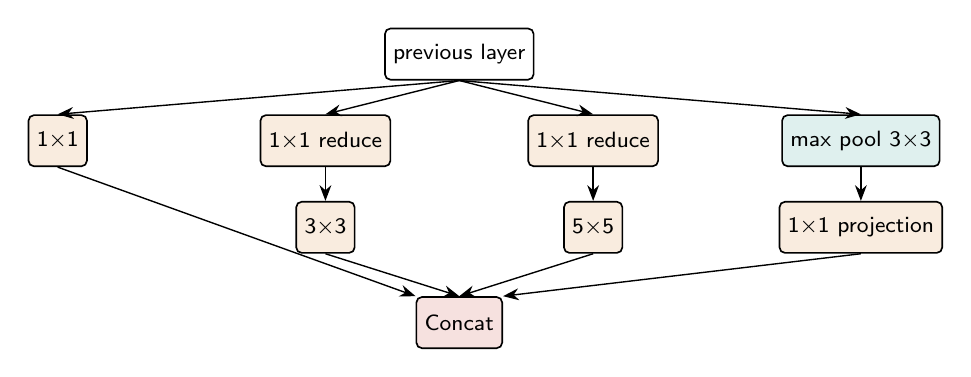
\begin{tikzpicture}[x=34mm, y=11mm]
  \node[blk] (in) at (1.5, 0) {previous layer};
  \node[blk, fill=nnconv!15] (a)  at (0, -1) {1$\times$1};
  \node[blk, fill=nnconv!15] (r3) at (1, -1) {1$\times$1 reduce};
  \node[blk, fill=nnconv!15] (r5) at (2, -1) {1$\times$1 reduce};
  \node[blk, fill=nnpool!15] (p)  at (3, -1) {max pool 3$\times$3};
  \node[blk, fill=nnconv!15] (c3) at (1, -2) {3$\times$3};
  \node[blk, fill=nnconv!15] (c5) at (2, -2) {5$\times$5};
  \node[blk, fill=nnconv!15] (pp) at (3, -2) {1$\times$1 projection};
  \node[blk, fill=nnjoin!15] (cat) at (1.5, -3.1) {Concat};
  \foreach \t in {a,r3,r5,p} \draw[arr] (in.south) -- (\t.north);
  \draw[arr] (r3) -- (c3); \draw[arr] (r5) -- (c5); \draw[arr] (p) -- (pp);
  \draw[arr] (a.south) -- (cat.north west);
  \foreach \t in {c3,c5} \draw[arr] (\t.south) -- (cat.north);
  \draw[arr] (pp.south) -- (cat.north east);
\end{tikzpicture}
\caption{An Inception module: four branches side by side (all keep the height and width); Concat stacks their channels.}
\end{figure}

\textbf{As built.} Stem: Conv2D 64 7$\times$7 stride 2, max pool, Conv2D 1$\times$1 64, Conv2D 3$\times$3 192, max pool (224
$\rightarrow$ 28). Then nine Inception modules with the paper's channel numbers: 3a (output 256 channels), 3b (480), max pool, 4a--4e
(512, 512, 512, 528, 832), max pool, 5a (832), 5b (1\,024); global average pooling, dropout 0.4, output. 5\,983\,802 parameters.

\textbf{Differences from the paper.} The two auxiliary classifiers used during training are left out (later work found them of little
use), and there is no local response normalisation.

\textbf{Training it.} 224$\times$224 inputs; without BatchNorm, deep plain networks like this train slowly: use Adam 0.0001--0.0003 and
patience, or add BatchNorm after the convolutions yourself.

%-------------------------------------------------------------------------------------------------------------------------------------
\subsection{ResNet-18 (2015)}
\textbf{Background.} Deeper plain networks became \emph{harder to train}, not just to generalise: adding layers raised the training error.
He et al.\ let every block learn a correction to its input, $y = x + F(x)$, through a shortcut~\cite{he2015resnet}; gradients then flow
through the shortcuts, and networks of 50, 101, even 1\,000 layers train well~\cite{he2016identity}.

\begin{figure}[htbp]\centering
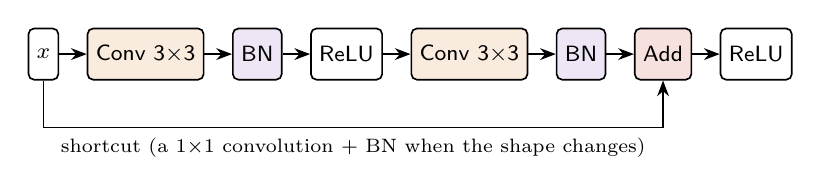
\begin{tikzpicture}[node distance=3.5mm]
  \node[blk] (x) {$x$};
  \node[blk, fill=nnconv!15, right=of x] (c1) {Conv 3$\times$3};
  \node[blk, fill=nnnorm!15, right=of c1] (b1) {BN};
  \node[blk, right=of b1] (r1) {ReLU};
  \node[blk, fill=nnconv!15, right=of r1] (c2) {Conv 3$\times$3};
  \node[blk, fill=nnnorm!15, right=of c2] (b2) {BN};
  \node[blk, fill=nnjoin!15, right=of b2] (add) {Add};
  \node[blk, right=of add] (r2) {ReLU};
  \foreach \a/\b in {x/c1,c1/b1,b1/r1,r1/c2,c2/b2,b2/add,add/r2} \draw[arr] (\a) -- (\b);
  \draw[arr] (x.south) -- ++(0,-6mm) -| (add.south);
  \node[font=\scriptsize] at ($(x.south)!0.5!(add.south) + (0,-8.5mm)$) {shortcut (a 1$\times$1 convolution + BN when the shape changes)};
\end{tikzpicture}
\caption{A basic residual block as built on the canvas: $y = \mathrm{ReLU}(x + F(x))$.}
\end{figure}

\textbf{As built.} Stem: Conv2D 64 7$\times$7 stride 2 + BatchNorm + ReLU, max pool 3$\times$3 stride 2 (224 $\rightarrow$ 56). Four
stages of two basic blocks with 64, 128, 256 and 512 filters; the first block of stages 2--4 has stride 2 and a 1$\times$1 stride-2
convolution with BatchNorm on the shortcut (56 $\rightarrow$ 28 $\rightarrow$ 14 $\rightarrow$ 7). Global average pooling and the output.
11\,181\,642 parameters, exactly torchvision's \texttt{resnet18} with a 10-class head.

\textbf{Training it.} The most forgiving of the large demos thanks to BatchNorm and the shortcuts. At 224$\times$224 it fits a T4 at batch
64--128. For CIFAR-10 at 32$\times$32 the stem shrinks the image too early (32 $\rightarrow$ 8 before the first block); the usual CIFAR
variant replaces the stem with a 3$\times$3 stride-1 convolution and drops the max pooling, an easy edit on the canvas.

%-------------------------------------------------------------------------------------------------------------------------------------
\subsection{MobileNet v1 (2017)}
\textbf{Background.} For phones, Howard et al.\ factorised a convolution into a \emph{depthwise} 3$\times$3 convolution (one filter per
channel, spatial only) and a \emph{pointwise} 1$\times$1 convolution (mixing channels)~\cite{howard2017mobilenets}. The cost drops by a
factor of about $1/N + 1/k^2$ ($N$ output channels, $k=3$): roughly eight to nine times fewer computations.

\textbf{As built.} Conv2D 32 3$\times$3 stride 2 + BN + ReLU, then 13 depthwise separable blocks (Depthwise Conv2D 3$\times$3 + BN +
ReLU, Conv2D 1$\times$1 + BN + ReLU) with 64, 128, 128, 256, 256, 512 ($\times$6), 1\,024, 1\,024 channels; five of them have stride 2
(224 $\rightarrow$ 7); global average pooling and the output. 3\,217\,226 parameters (4.2 million with 1\,000 classes, as in the paper).
Width and resolution multipliers of the paper can be imitated by changing the filter counts and the input size.

\textbf{Training it.} Light and fast; SGD or Adam 0.001 with BatchNorm works well. Depthwise convolutions are memory-bound on GPUs, so
it is not proportionally faster to \emph{train}; its advantage is at inference on small devices.

%-------------------------------------------------------------------------------------------------------------------------------------
\subsection{DenseNet, small CIFAR version (2017)}
\textbf{Background.} Huang et al.\ connected each layer to \emph{all} earlier layers of its block by concatenation~\cite{huang2016densenet}:
features are reused instead of re-learnt, so each layer can be narrow (the ``growth rate'' $k$, here 12 channels).

\textbf{As built.} Conv2D 24 3$\times$3; three dense blocks of four layers (BatchNorm $\rightarrow$ ReLU $\rightarrow$ Conv2D 12
3$\times$3, concatenated to everything before); between blocks a transition (BatchNorm $\rightarrow$ 1$\times$1 Conv2D halving the
channels $\rightarrow$ average pool 2$\times$2). The channels go 24 $\rightarrow$ 72 $\rightarrow$ 36 $\rightarrow$ 84 $\rightarrow$ 42
$\rightarrow$ 90 while the image goes 32 $\rightarrow$ 16 $\rightarrow$ 8; BatchNorm, ReLU, global pool and output. Only 76\,810 parameters.

\textbf{Differences from the paper.} The paper's CIFAR models are much deeper (for example 100 layers with bottleneck 1$\times$1
convolutions inside each layer, about 0.8 million parameters); the demo is a small teaching version. The paper's transitions have a ReLU
after their BatchNorm; the demo's do not.

\textbf{Training it.} CIFAR-10 built in, Adam 0.001, flips and crops, 50+ epochs; small but deep, so batch 64--128 fits easily.

%-------------------------------------------------------------------------------------------------------------------------------------
\subsection{Transformer encoder on image rows (2017)}
\textbf{Background.} The Transformer of Vaswani et al.\ replaced recurrence with self-attention: every token computes a weighted mix of
all tokens, the weights coming from query--key similarities~\cite{vaswani2017attention}. Its encoder is a stack of attention and
two-layer MLP blocks with residual connections and layer normalisation~\cite{ba2016layernorm}.

\textbf{As built.} A teaching version on MNIST: To tokens (\emph{rows}) makes each of the 28 rows a token of 28 values; Dense 64 embeds
them; Class token + position gives 29 tokens of 64; two pre-norm encoder blocks with 4 heads, an MLP of 128 (GELU~\cite{hendrycks2016gelu})
and dropout 0.1; LayerNorm, the class token, output. 71\,498 parameters.

\textbf{Training it.} MNIST, Adam 0.001, 10--20 epochs: it reaches high-90s accuracy and shows that attention can learn image structure
from a sequence of rows. Change the number of heads (64 must stay divisible by it) or blocks and compare.

%-------------------------------------------------------------------------------------------------------------------------------------
\subsection{ViT-Base/16 (2020)}
\textbf{Background.} Dosovitskiy et al.\ showed that a plain Transformer encoder on image patches, ``an image is worth 16$\times$16
words'', matches the best CNNs when pre-trained on enough data~\cite{dosovitskiy2020vit}.

\textbf{As built.} Conv2D 768 filters 16$\times$16 stride 16 (the patch embedding: 224 $\rightarrow$ 14$\times$14), To tokens (196 tokens
of 768), Class token + position (197 tokens), 12 encoder blocks (12 heads, MLP 3\,072), LayerNorm, class token, output.
85\,806\,346 parameters, exactly torchvision's \texttt{vit\_b\_16} with a 10-class head (86.6 million with 1\,000 classes).

\textbf{Training it.} ViTs lack the built-in assumptions of convolutions (locality, translation equivariance) and need much data or strong
augmentation and regularisation~\cite{steiner2021howtotrain,touvron2020deit}. From scratch on a small dataset it does worse than
ResNet-18. Use a low learning rate (0.0001 or less; AdamW with warm-up is the usual recipe~\cite{loshchilov2017adamw,goyal2017accurate},
not built in), batch 32--64 on a T4 with mixed precision.

%-------------------------------------------------------------------------------------------------------------------------------------
\subsection{ViT-Tiny for CIFAR-10}
\textbf{Background.} Small ViTs in the spirit of DeiT-Ti~\cite{touvron2020deit} (embedding 192, 3 heads) make transformers trainable
on small images in minutes.

\textbf{As built.} Conv2D 192 4$\times$4 stride 4 (32 $\rightarrow$ 8$\times$8 = 64 patches), To tokens, Class token + position (65
tokens), 6 encoder blocks with 3 heads, MLP 384 and dropout 0.1, LayerNorm, class token, output. 1\,806\,538 parameters. (DeiT-Ti itself
has 12 blocks and an MLP of 768.)

\textbf{Training it.} CIFAR-10 with flips and crops (augmentation matters a lot for ViTs), Adam 0.001 or a little lower, 50+ epochs. It
usually stays below the Small CNN on CIFAR-10 when trained from scratch for a short time: a useful experiment on the data hunger of
transformers.

%-------------------------------------------------------------------------------------------------------------------------------------
\subsection{ViT-g/14, one billion parameters (2022)}
\textbf{Background.} Zhai et al.\ studied how ViTs scale with model size, data and compute, training up to two billion parameters on
billions of images~\cite{zhai2021scaling}. ViT-g/14 (``giant'') is their one-billion-parameter model.

\textbf{As built.} Conv2D 1\,408 filters 14$\times$14 stride 14 (224 $\rightarrow$ 16$\times$16 = 256 patches), Class token + position
(257 tokens), 40 encoder blocks with 16 heads and MLP 6\,144, LayerNorm, class token, output: 1\,011\,216\,522 parameters. Each encoder
block alone has 25\,250\,176 parameters (attention $4d^2+4d$ = 7\,935\,488; MLP $2\cdot1408\cdot6144+6144+1408$ = 17\,309\,056; two
LayerNorms 5\,632). The canvas holds about 290 blocks; the layer table groups them into Embedding, 40 encoder blocks, Final norm and
Classifier.

\textbf{Training it.} About 16 GB of fixed state for Adam (Section~\ref{sec:math}): it does \emph{not} fit a 16 GB T4 (Kaggle,
g4dn.xlarge). A 48 GB RTX A6000 fits it with batches of roughly 16--32 at 224$\times$224 (estimate), at around 1.5 TFLOP of compute per
training image; a checkpoint with the optimiser state is about 12 GB and the final \file{model.pt} about 4 GB, both copied over the
network. From scratch on a small dataset it overfits badly and scores below ResNet-18; its value here is to see how a transformer scales
(compare it block by block with ViT-Base) and to measure memory and speed.

%-------------------------------------------------------------------------------------------------------------------------------------
\subsection{U-Net (2015)}
\textbf{Background.} Ronneberger et al.\ designed U-Net for biomedical image segmentation with few training images~\cite{ronneberger2015unet}:
a contracting path captures context, an expanding path recovers resolution, and skip connections hand the fine detail of each encoder
level to the decoder level of the same size.

\begin{figure}[htbp]\centering
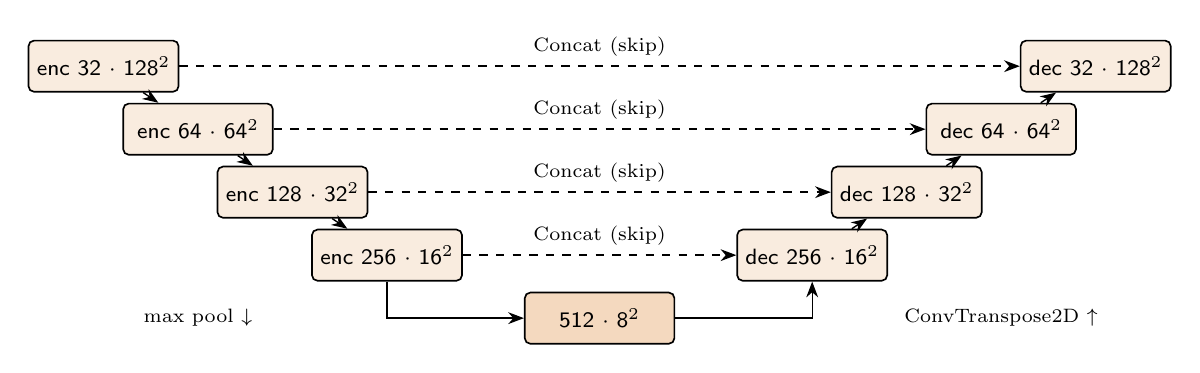
\begin{tikzpicture}[x=10mm, y=8mm]
  \foreach \i/\c/\s in {0/32/128,1/64/64,2/128/32,3/256/16} {
    \node[blk, fill=nnconv!15, minimum width=19mm] (e\i) at (\i*1.2, -\i) {enc \c\ $\cdot$ \s$^2$};
    \node[blk, fill=nnconv!15, minimum width=19mm] (d\i) at (12.6-\i*1.2, -\i) {dec \c\ $\cdot$ \s$^2$};
    \draw[arr, dashed] (e\i) -- node[above, font=\scriptsize] {Concat (skip)} (d\i);
  }
  \node[blk, fill=nnconv!30, minimum width=19mm] (b) at (6.3, -4) {512 $\cdot$ 8$^2$};
  \draw[arr] (e0) -- (e1); \draw[arr] (e1) -- (e2); \draw[arr] (e2) -- (e3); \draw[arr] (e3) |- (b);
  \draw[arr] (b) -| (d3); \draw[arr] (d3) -- (d2); \draw[arr] (d2) -- (d1); \draw[arr] (d1) -- (d0);
  \node[font=\scriptsize] at (1.2,-4) {max pool $\downarrow$};
  \node[font=\scriptsize] at (11.4,-4) {ConvTranspose2D $\uparrow$};
\end{tikzpicture}
\caption{The U shape as built: channels $\cdot$ image size per level, 128 $\rightarrow$ 8 pixels and back, with a skip at every level.}
\end{figure}

\textbf{As built.} Input 3$\times$128$\times$128. Encoder: four levels of two 3$\times$3 convolutions (ReLU) with 32, 64, 128, 256
filters, each followed by 2$\times$2 max pooling; bottleneck: two convolutions with 512 filters at 8$\times$8. Decoder: at each level a
2$\times$2 stride-2 ConvTranspose2D halving the channels, Concat with the encoder output of the same size, two 3$\times$3 convolutions;
Segmentation output (1$\times$1) with two classes. 7\,760\,130 parameters.

\textbf{Differences from the paper.} The paper starts at 64 filters (1\,024 at the bottom, about 31 million parameters) and uses
unpadded convolutions, cropping the encoder maps before concatenating; the demo uses padding ``same'', so sizes match without cropping.

\textbf{Training it.} Dataset $\rightarrow$ Segmentation, with an image column and a mask column (Hugging Face) or images and masks
folders (Kaggle); the class list maps mask values to classes. Flips and rotations are applied to the image and its mask together. Watch
the mIoU curve and the predicted masks in Results.

%-------------------------------------------------------------------------------------------------------------------------------------
\subsection{Attention U-Net (2018)}
\textbf{Background.} Oktay et al.\ added \emph{attention gates} to U-Net's skip connections: the decoder's coarser signal decides which
regions of the encoder features matter, suppressing irrelevant background~\cite{oktay2018attention}.

\textbf{As built.} U-Net as above, but before each Concat the skip features $x$ pass a gate: $g$ (the up-sampled decoder signal) and $x$
are each projected by a 1$\times$1 convolution to half the channels, added, passed through ReLU and a 1$\times$1 convolution to one channel
with a sigmoid; the resulting map $\psi\in[0,1]^{H\times W}$ multiplies $x$ (Multiply, one-channel map times image). 7\,847\,894 parameters.

\textbf{Difference from the paper.} The paper takes the gating signal from the coarser decoder level and resamples it; the demo uses the
up-sampled decoder features, which already have the skip's size.

%-------------------------------------------------------------------------------------------------------------------------------------
\subsection{MSG-Former: an NN Builder original}
\label{sec:msg}

MSG-Former (\emph{Multi-Scale Gated transFormer}) is the one demo that does not come from a paper: it was designed for NN Builder as a
small, fast network for 32$\times$32 colour images that combines three published ideas in one design. It is an untested proposal, not a
benchmark result: every number below (shapes, parameters, receptive fields, compute) is exact, but how well it classifies is for its
first training runs to show.

\subsubsection{The idea}
Convolutional networks and transformers are good at different things. A convolution looks at a small neighbourhood and is very efficient
at finding local texture and edges, but needs many layers before one output can relate two distant parts of the image. Self-attention
relates every position to every other in one step, but on raw pixels it is expensive and, without the built-in assumptions of
convolutions, needs much more data~\cite{dosovitskiy2020vit,touvron2020deit}. MSG-Former therefore works in two phases:
\begin{enumerate}
  \item \textbf{Local, multi-scale, gated} (32$\times$32 and 16$\times$16 pixels): convolution stages that look at three scales at once,
        weigh their channels by how useful they are, and keep a residual path;
  \item \textbf{Global} (an 8$\times$8 grid): the feature map becomes 64 tokens, and two Transformer encoder blocks let every region
        attend to every other before the class token makes the prediction.
\end{enumerate}
The same convolution-first, attention-later order is used by hybrid models such as the ResNet--ViT hybrid of the ViT
paper~\cite{dosovitskiy2020vit}, CoAtNet~\cite{dai2021coatnet} and MobileViT~\cite{mehta2021mobilevit}; MSG-Former's own contribution is the
form of its convolution stage.

\subsubsection{The multi-scale gated residual block}

\begin{figure}[htbp]\centering
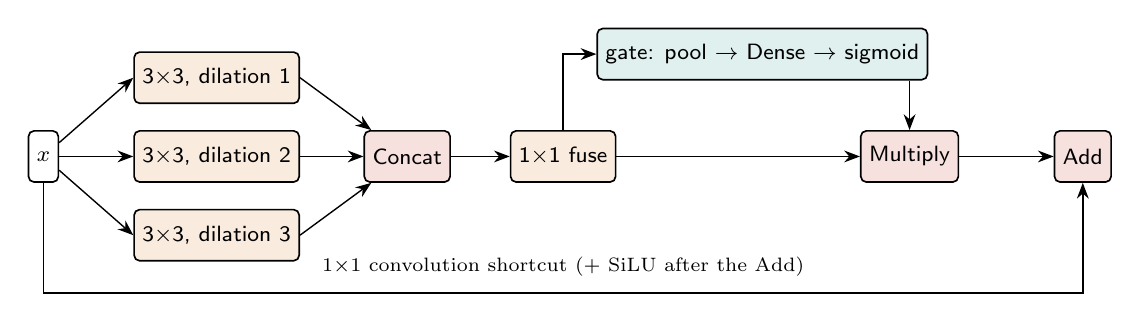
\begin{tikzpicture}[x=22mm, y=10mm]
  \node[blk] (x) at (0, 0) {$x$};
  \node[blk, fill=nnconv!15] (d1) at (1, 1) {3$\times$3, dilation 1};
  \node[blk, fill=nnconv!15] (d2) at (1, 0) {3$\times$3, dilation 2};
  \node[blk, fill=nnconv!15] (d3) at (1, -1) {3$\times$3, dilation 3};
  \node[blk, fill=nnjoin!15] (cat) at (2.1, 0) {Concat};
  \node[blk, fill=nnconv!15] (f) at (3, 0) {1$\times$1 fuse};
  \node[blk, fill=nnpool!15] (se) at (4.15, 1.3) {gate: pool $\rightarrow$ Dense $\rightarrow$ sigmoid};
  \node[blk, fill=nnjoin!15] (m) at (5, 0) {Multiply};
  \node[blk, fill=nnjoin!15] (add) at (6, 0) {Add};
  \foreach \t in {d1,d2,d3} {\draw[arr] (x) -- (\t.west); \draw[arr] (\t.east) -- (cat);}
  \draw[arr] (cat) -- (f); \draw[arr] (f) -- (m);
  \draw[arr] (f.north) |- (se.west); \draw[arr] (se.south -| m.north) -- (m.north);
  \draw[arr] (m) -- (add);
  \draw[arr] (x.south) -- ++(0,-14mm) -| (add.south);
  \node[font=\scriptsize, fill=white, inner sep=1pt] at (3, -1.4) {1$\times$1 convolution shortcut (+ SiLU after the Add)};
\end{tikzpicture}
\caption{The multi-scale gated residual block. Each 3$\times$3 branch is Conv2D (no bias) $\rightarrow$ BatchNorm $\rightarrow$ SiLU; the
fuse is a 1$\times$1 Conv2D $\rightarrow$ BatchNorm $\rightarrow$ ReLU; the gate is Global pool $\rightarrow$ Dense ($C/4$, ReLU)
$\rightarrow$ Dense ($C$, sigmoid).}
\label{fig:msgblock}
\end{figure}

For an input $x$ with $C_{\text{in}}$ channels, a branch width $b$ and an output width $C$, the block computes
\begin{align}
  u_r &= \operatorname{SiLU}\bigl(\operatorname{BN}(W_r \ast_r x)\bigr), \qquad r \in \{1, 2, 3\}\quad(\ast_r:\ \text{3$\times$3 convolution with dilation } r),\\
  v &= \operatorname{ReLU}\bigl(\operatorname{BN}(W_f \ast [u_1; u_2; u_3])\bigr) \qquad (\text{1$\times$1 fuse of the $3b$ concatenated channels to } C),\\
  g &= \sigma\bigl(W_2\, \operatorname{ReLU}(W_1\, \operatorname{GAP}(v) + c_1) + c_2\bigr) \in (0,1)^{C},\\
  y &= \operatorname{SiLU}\bigl(g \odot v + W_s \ast x\bigr) \qquad (W_s:\ \text{1$\times$1 shortcut, } C_{\text{in}} \rightarrow C).
\end{align}
Each part has a reason:
\begin{description}
  \item[Three dilations, same cost.] A 3$\times$3 kernel with dilation $r$ covers $(2r+1)\times(2r+1)$ pixels with the same nine weights:
        3$\times$3, 5$\times$5 and 7$\times$7 here~\cite{yu2015dilated}. The block sees fine detail and wider context at the same
        resolution and the price of three ordinary 3$\times$3 convolutions, like an Inception module~\cite{szegedy2014going} without
        the cost of large kernels, or the atrous spatial pyramid of DeepLab~\cite{chen2017deeplabv3} inside a classifier. Mixing the
        rates 1, 2 and 3 (rather than only large ones) keeps every pixel covered and avoids the ``gridding'' gaps that stacked dilated
        convolutions can leave~\cite{wang2017hdc}.
  \item[1$\times$1 fuse.] Concatenation gives $3b$ channels; the 1$\times$1 convolution mixes the scales and sets the block's width.
  \item[Squeeze-and-excitation gate.] Global average pooling summarises each channel over the whole image; two small Dense layers
        (reduction 4) turn that summary into one weight in $(0,1)$ per channel, and Multiply scales the channels with it, so the block can
        emphasise the scales and features that matter for this image~\cite{hu2017senet}. The original SE networks use reduction 16;
        with 64 and 128 channels, 4 keeps the bottleneck from becoming too narrow (16 and 32 units).
  \item[Residual shortcut.] As in ResNet~\cite{he2015resnet}, the block learns a correction to its input; because the channel count
        changes (32 $\rightarrow$ 64, 64 $\rightarrow$ 128), the shortcut is a 1$\times$1 projection.
  \item[SiLU.] A smooth activation~\cite{ramachandran2017swish} in the branches and after the sum; the fuse keeps ReLU.
\end{description}

\subsubsection{The whole network}

\begin{figure}[htbp]\centering
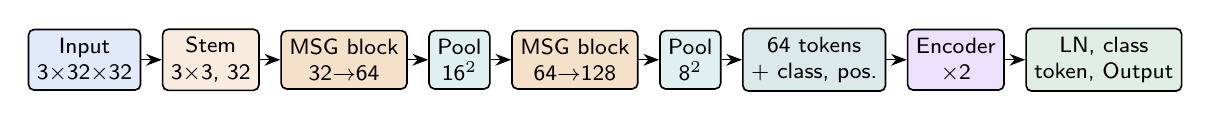
\begin{tikzpicture}[node distance=2.6mm, every node/.append style={font=\scriptsize\sffamily}]
  \node[blk, fill=nnin!15, align=center] (in) {Input\\3$\times$32$\times$32};
  \node[blk, fill=nnconv!15, right=of in, align=center] (stem) {Stem\\3$\times$3, 32};
  \node[blk, fill=nnconv!25, right=of stem, align=center] (b1) {MSG block\\32$\rightarrow$64};
  \node[blk, fill=nnpool!15, right=of b1, align=center] (p1) {Pool\\16$^2$};
  \node[blk, fill=nnconv!25, right=of p1, align=center] (b2) {MSG block\\64$\rightarrow$128};
  \node[blk, fill=nnpool!15, right=of b2, align=center] (p2) {Pool\\8$^2$};
  \node[blk, fill=nntok!15, right=of p2, align=center] (tk) {64 tokens\\+ class, pos.};
  \node[blk, fill=nnatt!15, right=of tk, align=center] (enc) {Encoder\\$\times$2};
  \node[blk, fill=nnout!15, right=of enc, align=center] (out) {LN, class\\token, Output};
  \foreach \a/\b in {in/stem,stem/b1,b1/p1,p1/b2,b2/p2,p2/tk,tk/enc,enc/out} \draw[arr] (\a) -- (\b);
\end{tikzpicture}
\caption{MSG-Former from left to right: local multi-scale stages at 32$\times$32 and 16$\times$16, then global attention on an 8$\times$8 grid.}
\label{fig:msgall}
\end{figure}

\screenshot{04_design_msg_zoom}{MSG-Former on the canvas, zoomed in on the first block: the stem's activation feeds the three dilated
3$\times$3 convolutions (dilation 1, 2, 3, each with BatchNorm and SiLU) and, at the bottom, the 1$\times$1 shortcut; the branches meet in
Concat (96 channels). Every arrow shows its tensor shape.}{fig:msgcanvas}

\screenshot{03_design_msg}{The whole design opened from the demo: 72 blocks, 466\,522 parameters, ``ready''. The layer table groups them
as Input, Stage~1 $\cdot$ 32$\times$32, Stage~2 $\cdot$ 16$\times$16, Embedding, Encoder block 1 and 2, Final norm and Classifier, each
with its output, parameters and receptive field.}{fig:msgtable}

Table~\ref{tab:msglayers} lists every layer as the application computes it (with 10 classes). The receptive field (RF) is given in
input pixels.

{\small
\begin{longtable}{@{}p{1.8cm}p{5.5cm}lrr@{}}
\caption{MSG-Former layer by layer.}\label{tab:msglayers}\\
\toprule
\textbf{Stage} & \textbf{Layer} & \textbf{Output} & \textbf{Parameters} & \textbf{RF}\\
\midrule\endfirsthead
\toprule
\textbf{Stage} & \textbf{Layer} & \textbf{Output} & \textbf{Parameters} & \textbf{RF}\\
\midrule\endhead
Input & image & 3$\times$32$\times$32 & 0 & 1\\
Stem & Conv2D 32, 3$\times$3, no bias; BatchNorm; ReLU & 32$\times$32$\times$32 & 864 + 64 & 3\\
Block 1 & branch $r=1$: Conv2D 32 3$\times$3; BatchNorm; SiLU & 32$\times$32$\times$32 & 9\,216 + 64 & 5\\
 & branch $r=2$: Conv2D 32 3$\times$3 dilation 2; BatchNorm; SiLU & 32$\times$32$\times$32 & 9\,216 + 64 & 7\\
 & branch $r=3$: Conv2D 32 3$\times$3 dilation 3; BatchNorm; SiLU & 32$\times$32$\times$32 & 9\,216 + 64 & 9\\
 & Concat & 96$\times$32$\times$32 & 0 & 9\\
 & fuse: Conv2D 64 1$\times$1; BatchNorm; ReLU & 64$\times$32$\times$32 & 6\,144 + 128 & 9\\
 & gate: Global pool; Dense 16 ReLU; Dense 64 sigmoid & 64 & 1\,040 + 1\,088 & \\
 & Multiply (gate $\times$ fused map) & 64$\times$32$\times$32 & 0 & \\
 & shortcut: Conv2D 64 1$\times$1, no bias & 64$\times$32$\times$32 & 2\,048 & \\
 & Add; SiLU & 64$\times$32$\times$32 & 0 & \\
 & Pool max 2$\times$2 & 64$\times$16$\times$16 & 0 & 10\\
Block 2 & branches $r=1,2,3$: Conv2D 64 3$\times$3; BatchNorm; SiLU & 3 $\times$ 64$\times$16$\times$16 & 3 $\times$ (36\,864 + 128) & 14, 18, 22\\
 & Concat & 192$\times$16$\times$16 & 0 & 22\\
 & fuse: Conv2D 128 1$\times$1; BatchNorm; ReLU & 128$\times$16$\times$16 & 24\,576 + 256 & 22\\
 & gate: Global pool; Dense 32 ReLU; Dense 128 sigmoid & 128 & 4\,128 + 4\,224 & \\
 & Multiply; shortcut Conv2D 128 1$\times$1; Add; SiLU & 128$\times$16$\times$16 & 8\,192 & \\
 & Pool max 2$\times$2 & 128$\times$8$\times$8 & 0 & 24\\
Embedding & To tokens (patches): every cell of the 8$\times$8 map & 64$\times$128 & 0 & \\
 & Class token + position embeddings & 65$\times$128 & 8\,448 & \\
Encoder 1 & LayerNorm; Self-attention (4 heads, dropout 0.1); Dropout; Add & 65$\times$128 & 256 + 66\,048 & global\\
 & LayerNorm; Dense 256 GELU; Dropout; Dense 128; Dropout; Add & 65$\times$128 & 256 + 33\,024 + 32\,896 & \\
Encoder 2 & the same & 65$\times$128 & 132\,480 & \\
Head & LayerNorm; Token pool (class token); Dropout 0.2; Output & 10 & 256 + 1\,290 & \\
\midrule
 & \textbf{Total} & & \textbf{466\,522} & \\
\bottomrule
\end{longtable}}

\paragraph{Where the parameters are.}
\begin{center}
\begin{tabularx}{\linewidth}{@{}Xrr@{}}
\toprule
\textbf{Part} & \textbf{Parameters} & \textbf{Share}\\
\midrule
Stem & 928 & 0.2\%\\
Block 1 (branches 27\,840, fuse 6\,272, gate 2\,128, shortcut 2\,048) & 38\,288 & 8.2\%\\
Block 2 (branches 110\,976, fuse 24\,832, gate 8\,352, shortcut 8\,192) & 152\,352 & 32.7\%\\
Class token and positions & 8\,448 & 1.8\%\\
Two encoder blocks (attention 66\,048, MLP 65\,920, norms 512 each) & 264\,960 & 56.8\%\\
Final LayerNorm and output & 1\,546 & 0.3\%\\
\midrule
Total & 466\,522 & 100\%\\
\bottomrule
\end{tabularx}
\end{center}
These counts were derived by hand, agree with the application's engine, are pinned in its automatic tests, and are confirmed against a
real PyTorch build of the network on every change (the comparison on GitHub, Section~\ref{sec:math}).

\paragraph{Where the computation is.}
Counting multiply--accumulate operations (MACs) of the convolutions, the Dense layers and attention for one 32$\times$32 image (BatchNorm,
activations and pooling are negligible):
\begin{center}
\begin{tabularx}{\linewidth}{@{}Xr@{}}
\toprule
\textbf{Part} & \textbf{MACs per image}\\
\midrule
Stem ($9\cdot3\cdot32\cdot32^2$) & 0.88 M\\
Block 1: branches $3\cdot(9\cdot32\cdot32\cdot32^2)$ 28.3 M, fuse 6.3 M, shortcut 2.1 M & 36.7 M\\
Block 2: branches $3\cdot(9\cdot64\cdot64\cdot16^2)$ 28.3 M, fuse 6.3 M, shortcut 2.1 M & 36.7 M\\
Encoders: per block projections $4Nd^2$ 4.3 M, attention $2N^2d$ 1.1 M, MLP $2Nd\cdot256$ 4.3 M ($N=65$, $d=128$) & 19.2 M\\
\midrule
Total & about 93.5 M\\
\bottomrule
\end{tabularx}
\end{center}
About 94 million multiply--accumulates (roughly 0.19 GFLOP) per image: the convolution stages do about 80\% of the work with about 41\% of
the parameters, the encoders the reverse (21\% of the work, 57\% of the parameters). Because pooling halves the image before block 2 while
the width doubles, both blocks cost almost exactly the same. Attention is cheap here because there are only 65 tokens: its $N^2$ term is
1.1 M MACs per block. Training costs about three times the forward pass, so one epoch of CIFAR-10 (50\,000 images) is roughly
$1.4\times10^{13}$ MACs, a few minutes on a T4.

\paragraph{Receptive field.}
Before the transformer each token sees a 24$\times$24 pixel region of the 32$\times$32 image (the RF column of
Table~\ref{tab:msglayers}), and neighbouring tokens are 4 pixels apart, so their regions overlap heavily. The first encoder block then makes
the receptive field global: every token, and the class token, can draw on every part of the image.

\subsubsection{Training it}
\begin{enumerate}
  \item Open MSG-Former from the Projects page and save it (\kbd{Cmd+S}). It opens with built-in CIFAR-10 at its own size.
  \item Train tab: Adam, learning rate 0.001 (0.0005 if the loss is unstable), batch 128, 30--60 epochs; augmentation: horizontal flip
        and random crop with 4 pixels of padding (transformer layers in particular profit from augmentation~\cite{steiner2021howtotrain}).
  \item Train on Kaggle or any GPU: by a rough estimate it needs about 1 GB of GPU memory at batch 128 (mostly the activations of the two
        convolution stages kept for the backward pass), so even small GPUs are enough.
  \item Compare with the Small CNN (551\,018 parameters, convolution only) and ViT-Tiny (1\,806\,538 parameters, attention only), trained
        with the same settings, in the Runs table.
\end{enumerate}

\subsubsection{Experiments to run (ablations)}
Each is a small edit on the canvas, and together they show which part of the design earns its place:
\begin{center}
\begin{tabularx}{\linewidth}{@{}lXr@{}}
\toprule
& \textbf{Change on the canvas} & \textbf{Parameters}\\
\midrule
A & Remove both gates (delete Global pool, the two Dense layers and Multiply; connect the fuse to Add) & 456\,042\\
B & All dilations 1 (three identical-scale branches) & 466\,522\\
C & No transformer: Global pool after the second pooling, then Output & 192\,858\\
D & A third encoder block & 598\,970\\
E & Token pool \emph{mean} instead of the class token & 466\,522\\
F & Wider: branch filters 64 and 128 & larger\\
\bottomrule
\end{tabularx}
\end{center}
(Counts for A, C and D follow from the tables above: A removes $2\,128+8\,352$; C removes the embedding, encoders, final norm and the
128-input head and adds a 128-input head; D adds one encoder block of 132\,480. The application shows the exact count after each edit.)
If B matches the full model, the multi-scale branches are not helping on this data; if C matches it, the attention is not; and so on.

\subsubsection{Adapting it}
\begin{itemize}
  \item \textbf{Larger images} (for example 64$\times$64 or 224$\times$224): add a stride-2 stem (or a third block with pooling) so that
        the grid reaching the transformer stays around 8$\times$8 to 14$\times$14; otherwise the number of tokens, and the $N^2$ attention
        cost, grows with the image.
  \item \textbf{More classes:} only the output layer changes ($128\cdot K + K$ parameters).
  \item \textbf{Segmentation:} the two convolution stages can serve as an encoder in a U-Net-style design, with ConvTranspose2D decoders
        and skips from the blocks.
\end{itemize}

\subsubsection{Status}
The design, its shapes and its parameter count are verified (by hand, by the application's engine and against PyTorch). Its accuracy is
not: no training results exist yet. Treat it as a starting point for experiments, and record the results of the comparisons above.

%=====================================================================================================================================
\section{Troubleshooting}

\begin{description}
  \item[``design has problems''.] Open Design; the red block says why (Section~\ref{sec:checks}). Blocks after it are greyed out until it is fixed.
  \item[``dataset incomplete'' or no classes.] The class list is empty (Hugging Face: \ui{Read info} and a ClassLabel column; Kaggle:
        type the class folder names). Text datasets cannot be used.
  \item[The one-batch check stops the run.] A layer's real shape differed from the application's (for example images of an unexpected
        size in a custom dataset). The message names the layer; check the image size and channels in the Dataset tab.
  \item[``CUDA out of memory''.] With \ui{Split a batch that does not fit} on (the default) the run handles this itself and continues
        more slowly. If even one image at a time does not fit, the run stops with a message: switch on \ui{Save memory}, keep mixed
        precision on, or use a smaller input size, network or a larger GPU (Section~\ref{sec:math}).
  \item[Kaggle run fails to start.] The account must be phone-verified for GPU and internet access; the token must be current.
  \item[SSH machine does not answer.] Password machines: press \ui{Connect} again (the login lasts a few hours); key machines:
        \ui{Test}. A running training is not affected.
  \item[EC2: ``no public address'' / ssh never answers.] Give the instance a public IP (or an Elastic IP), allow port 22 in its security
        group, and use its key file. A new account may have a vCPU quota of 0 for G instances: request an increase.
  \item[EC2 spot: the run says ``interrupted''.] AWS took the capacity back; with a persistent request and behaviour \emph{stop} it resumes
        by itself. To continue now, use \ui{Continue on another machine} (needs the checkpoint copy on the Mac).
  \item[A demo disappeared.] Unsaved demos are discarded when another demo or project is opened or the application quits; save them with
        \kbd{Cmd+S}.
  \item[Training is unstable (loss jumps or becomes NaN).] Lower the learning rate (by 10$\times$), keep mixed precision on (the script
        scales the loss), add BatchNorm / LayerNorm, check that the labels match the class list.
  \item[High training accuracy, low validation accuracy.] Overfitting: augmentation, dropout, fewer parameters (Global pool instead of
        Flatten + large Dense), more data, fewer epochs.
\end{description}

%=====================================================================================================================================
\section{Privacy and security}
\begin{itemize}
  \item Tokens and keys live only in the system keychain; they are passed to one call at a time, and written on a remote machine only
        when a run needs them, as files readable by their owner.
  \item The design computer never downloads datasets or runs training; it reads dataset descriptions only.
  \item Unsaved demos are kept in the application's own folder and deleted when no longer needed; projects live where you choose.
  \item Updates come only from the project's GitHub releases and are checked against the published SHA-256 checksum.
\end{itemize}

%=====================================================================================================================================
\appendix
\section{Glossary}
\begin{description}[itemsep=1pt]
  \item[Activation function] a non-linear function applied element-wise (ReLU, GELU, \ldots).
  \item[Batch] the images processed together in one training step.
  \item[Channel] one ``layer'' of an image or feature map (3 for RGB; a convolution with 64 filters produces 64).
  \item[Checkpoint] a saved training state (weights, optimiser, position) from which a run can resume.
  \item[Epoch] one pass over the whole training set.
  \item[Feature map] the output of a convolution: one image per filter.
  \item[Kernel / filter] the small window of weights a convolution slides over the image.
  \item[mIoU] mean over the classes of (overlap / union) of predicted and true masks.
  \item[Padding] pixels added around the image so the window can reach the borders.
  \item[Parameter] a trainable number (weight or bias).
  \item[Receptive field] the input region one output value depends on.
  \item[Spot instance] spare cloud capacity at a lower price that the provider can take back.
  \item[Stride] how far the window moves at each step.
  \item[Token] one element of a sequence a transformer works on (here: an image patch or row).
\end{description}

%=====================================================================================================================================
\begin{thebibliography}{99}\small

\bibitem{ba2016layernorm} J.~L. Ba, J.~R. Kiros and G.~E. Hinton. Layer normalization. 2016.
  \href{https://arxiv.org/abs/1607.06450}{arXiv:1607.06450}.
\bibitem{chen2017deeplabv3} L.-C. Chen, G.~Papandreou, F.~Schroff and H.~Adam. Rethinking atrous convolution for semantic image
  segmentation. 2017. \href{https://arxiv.org/abs/1706.05587}{arXiv:1706.05587}.
\bibitem{chen2016checkpoint} T.~Chen, B.~Xu, C.~Zhang and C.~Guestrin. Training deep nets with sublinear memory cost. 2016.
  \href{https://arxiv.org/abs/1604.06174}{arXiv:1604.06174}.
\bibitem{cubuk2018autoaugment} E.~D. Cubuk, B.~Zoph, D.~Man\'e, V.~Vasudevan and Q.~V. Le. AutoAugment: learning augmentation policies
  from data. 2018. \href{https://arxiv.org/abs/1805.09501}{arXiv:1805.09501}.
\bibitem{dai2021coatnet} Z.~Dai, H.~Liu, Q.~V. Le and M.~Tan. CoAtNet: marrying convolution and attention for all data sizes. 2021.
  \href{https://arxiv.org/abs/2106.04803}{arXiv:2106.04803}.
\bibitem{dosovitskiy2020vit} A.~Dosovitskiy et al. An image is worth 16x16 words: Transformers for image recognition at scale. 2020.
  \href{https://arxiv.org/abs/2010.11929}{arXiv:2010.11929}.
\bibitem{dumoulin2016guide} V.~Dumoulin and F.~Visin. A guide to convolution arithmetic for deep learning. 2016.
  \href{https://arxiv.org/abs/1603.07285}{arXiv:1603.07285}.
\bibitem{goyal2017accurate} P.~Goyal et al. Accurate, large minibatch SGD: training ImageNet in 1 hour. 2017.
  \href{https://arxiv.org/abs/1706.02677}{arXiv:1706.02677}.
\bibitem{he2015resnet} K.~He, X.~Zhang, S.~Ren and J.~Sun. Deep residual learning for image recognition. 2015.
  \href{https://arxiv.org/abs/1512.03385}{arXiv:1512.03385}.
\bibitem{he2016identity} K.~He, X.~Zhang, S.~Ren and J.~Sun. Identity mappings in deep residual networks. 2016.
  \href{https://arxiv.org/abs/1603.05027}{arXiv:1603.05027}.
\bibitem{hendrycks2016gelu} D.~Hendrycks and K.~Gimpel. Gaussian error linear units (GELUs). 2016.
  \href{https://arxiv.org/abs/1606.08415}{arXiv:1606.08415}.
\bibitem{hinton2012dropout} G.~E. Hinton, N.~Srivastava, A.~Krizhevsky, I.~Sutskever and R.~R. Salakhutdinov. Improving neural networks
  by preventing co-adaptation of feature detectors. 2012. \href{https://arxiv.org/abs/1207.0580}{arXiv:1207.0580}.
\bibitem{howard2017mobilenets} A.~G. Howard et al. MobileNets: efficient convolutional neural networks for mobile vision applications.
  2017. \href{https://arxiv.org/abs/1704.04861}{arXiv:1704.04861}.
\bibitem{hu2017senet} J.~Hu, L.~Shen, S.~Albanie, G.~Sun and E.~Wu. Squeeze-and-excitation networks. 2017.
  \href{https://arxiv.org/abs/1709.01507}{arXiv:1709.01507}.
\bibitem{huang2016densenet} G.~Huang, Z.~Liu, L.~van der Maaten and K.~Q. Weinberger. Densely connected convolutional networks. 2016.
  \href{https://arxiv.org/abs/1608.06993}{arXiv:1608.06993}.
\bibitem{ioffe2015batchnorm} S.~Ioffe and C.~Szegedy. Batch normalization: accelerating deep network training by reducing internal
  covariate shift. 2015. \href{https://arxiv.org/abs/1502.03167}{arXiv:1502.03167}.
\bibitem{kingma2014adam} D.~P. Kingma and J.~Ba. Adam: a method for stochastic optimization. 2014.
  \href{https://arxiv.org/abs/1412.6980}{arXiv:1412.6980}.
\bibitem{krizhevsky2009cifar} A.~Krizhevsky. Learning multiple layers of features from tiny images. Technical report, University of
  Toronto, 2009 (not on arXiv). \url{https://www.cs.toronto.edu/~kriz/learning-features-2009-TR.pdf}.
\bibitem{krizhevsky2012alexnet} A.~Krizhevsky, I.~Sutskever and G.~E. Hinton. ImageNet classification with deep convolutional neural
  networks. NeurIPS 2012 (not on arXiv).
  \url{https://papers.nips.cc/paper/2012/hash/c399862d3b9d6b76c8436e924a68c45b-Abstract.html}.
\bibitem{krizhevsky2014weird} A.~Krizhevsky. One weird trick for parallelizing convolutional neural networks. 2014.
  \href{https://arxiv.org/abs/1404.5997}{arXiv:1404.5997}.
\bibitem{lecun1998gradient} Y.~LeCun, L.~Bottou, Y.~Bengio and P.~Haffner. Gradient-based learning applied to document recognition.
  Proceedings of the IEEE 86(11), 1998 (not on arXiv). \href{https://doi.org/10.1109/5.726791}{doi:10.1109/5.726791}.
\bibitem{lhoest2021datasets} Q.~Lhoest et al. Datasets: a community library for natural language processing. 2021.
  \href{https://arxiv.org/abs/2109.02846}{arXiv:2109.02846}.
\bibitem{lin2013nin} M.~Lin, Q.~Chen and S.~Yan. Network in network. 2013.
  \href{https://arxiv.org/abs/1312.4400}{arXiv:1312.4400}.
\bibitem{loshchilov2017adamw} I.~Loshchilov and F.~Hutter. Decoupled weight decay regularization. 2017.
  \href{https://arxiv.org/abs/1711.05101}{arXiv:1711.05101}.
\bibitem{luo2017erf} W.~Luo, Y.~Li, R.~Urtasun and R.~Zemel. Understanding the effective receptive field in deep convolutional neural
  networks. 2017. \href{https://arxiv.org/abs/1701.04128}{arXiv:1701.04128}.
\bibitem{mehta2021mobilevit} S.~Mehta and M.~Rastegari. MobileViT: light-weight, general-purpose, and mobile-friendly Vision
  Transformer. 2021. \href{https://arxiv.org/abs/2110.02178}{arXiv:2110.02178}.
\bibitem{micikevicius2017mixed} P.~Micikevicius et al. Mixed precision training. 2017.
  \href{https://arxiv.org/abs/1710.03740}{arXiv:1710.03740}.
\bibitem{oktay2018attention} O.~Oktay et al. Attention U-Net: learning where to look for the pancreas. 2018.
  \href{https://arxiv.org/abs/1804.03999}{arXiv:1804.03999}.
\bibitem{paszke2019pytorch} A.~Paszke et al. PyTorch: an imperative style, high-performance deep learning library. 2019.
  \href{https://arxiv.org/abs/1912.01703}{arXiv:1912.01703}.
\bibitem{rajbhandari2019zero} S.~Rajbhandari, J.~Rasley, O.~Ruwase and Y.~He. ZeRO: memory optimizations toward training trillion
  parameter models. 2019. \href{https://arxiv.org/abs/1910.02054}{arXiv:1910.02054}.
\bibitem{ramachandran2017swish} P.~Ramachandran, B.~Zoph and Q.~V. Le. Searching for activation functions. 2017.
  \href{https://arxiv.org/abs/1710.05941}{arXiv:1710.05941}.
\bibitem{ronneberger2015unet} O.~Ronneberger, P.~Fischer and T.~Brox. U-Net: convolutional networks for biomedical image segmentation.
  2015. \href{https://arxiv.org/abs/1505.04597}{arXiv:1505.04597}.
\bibitem{russakovsky2014imagenet} O.~Russakovsky et al. ImageNet large scale visual recognition challenge. 2014.
  \href{https://arxiv.org/abs/1409.0575}{arXiv:1409.0575}.
\bibitem{selvaraju2016gradcam} R.~R. Selvaraju et al. Grad-CAM: visual explanations from deep networks via gradient-based localization.
  2016. \href{https://arxiv.org/abs/1610.02391}{arXiv:1610.02391}.
\bibitem{simonyan2014vgg} K.~Simonyan and A.~Zisserman. Very deep convolutional networks for large-scale image recognition. 2014.
  \href{https://arxiv.org/abs/1409.1556}{arXiv:1409.1556}.
\bibitem{srivastava2014dropout} N.~Srivastava, G.~Hinton, A.~Krizhevsky, I.~Sutskever and R.~Salakhutdinov. Dropout: a simple way to
  prevent neural networks from overfitting. JMLR 15, 2014 (not on arXiv; see also \cite{hinton2012dropout}).
  \url{https://jmlr.org/papers/v15/srivastava14a.html}.
\bibitem{steiner2021howtotrain} A.~Steiner et al. How to train your ViT? Data, augmentation, and regularization in Vision Transformers.
  2021. \href{https://arxiv.org/abs/2106.10270}{arXiv:2106.10270}.
\bibitem{szegedy2014going} C.~Szegedy et al. Going deeper with convolutions. 2014.
  \href{https://arxiv.org/abs/1409.4842}{arXiv:1409.4842}.
\bibitem{touvron2020deit} H.~Touvron et al. Training data-efficient image transformers \& distillation through attention. 2020.
  \href{https://arxiv.org/abs/2012.12877}{arXiv:2012.12877}.
\bibitem{vaswani2017attention} A.~Vaswani et al. Attention is all you need. 2017.
  \href{https://arxiv.org/abs/1706.03762}{arXiv:1706.03762}.
\bibitem{wang2017hdc} P.~Wang et al. Understanding convolution for semantic segmentation. 2017.
  \href{https://arxiv.org/abs/1702.08502}{arXiv:1702.08502}.
\bibitem{xiao2017fashion} H.~Xiao, K.~Rasul and R.~Vollgraf. Fashion-MNIST: a novel image dataset for benchmarking machine learning
  algorithms. 2017. \href{https://arxiv.org/abs/1708.07747}{arXiv:1708.07747}.
\bibitem{xiong2020prenorm} R.~Xiong et al. On layer normalization in the Transformer architecture. 2020.
  \href{https://arxiv.org/abs/2002.04745}{arXiv:2002.04745}.
\bibitem{yu2015dilated} F.~Yu and V.~Koltun. Multi-scale context aggregation by dilated convolutions. 2015.
  \href{https://arxiv.org/abs/1511.07122}{arXiv:1511.07122}.
\bibitem{zhai2021scaling} X.~Zhai, A.~Kolesnikov, N.~Houlsby and L.~Beyer. Scaling Vision Transformers. 2021.
  \href{https://arxiv.org/abs/2106.04560}{arXiv:2106.04560}.

\bibitem{garnot2021utae} V.~Sainte Fare Garnot and L.~Landrieu. Panoptic segmentation of satellite image time series with convolutional
temporal attention networks. ICCV, 2021. arXiv:2107.07933.
\bibitem{tarasiou2023tsvit} M.~Tarasiou, E.~Chavez and S.~Zafeiriou. ViTs for SITS: Vision transformers for satellite image time series. CVPR,
2023. arXiv:2301.04944.
\bibitem{hochreiter1997lstm} S.~Hochreiter and J.~Schmidhuber. Long short-term memory. Neural Computation 9(8), 1997.
\bibitem{zhou2019centernet} X.~Zhou, D.~Wang and P.~Kr\"ahenb\"uhl. Objects as points. 2019. arXiv:1904.07850.
\bibitem{hu2021lora} E.~J.~Hu, Y.~Shen, P.~Wallis et al. LoRA: Low-rank adaptation of large language models. 2021. arXiv:2106.09685.
\end{thebibliography}

\end{document}
